%%%%%%%%%%%%%%%%%%%%%%%%%%%%%%%%%%%%%%%%%%%%%%%%%%%%%%%%%%%%%%%%%%%%%%%%%%%%%%
% Modello semplice Logistic Regression
%%%%%%%%%%%%%%%%%%%%%%%%%%%%%%%%%%%%%%%%%%%%%%%%%%%%%%%%%%%%%%%%%%%%%%%%%%%%%%

\subsection{Modello semplice Logistic Regression}

\subsection*{Smoke}
\begin{center}
\begin{minipage}[c]{0.50\columnwidth}
\resizebox{\columnwidth}{!}{%
\begin{tabular}{lcccc}
\toprule
Label        & Precision & Recall & F1-score & Support \\
\midrule
Non-smoker   & 0.69      & 0.91   & 0.79     & 167528 \\
Ex-smoker    & 0.40      & 0.09   & 0.15     & 47377  \\
Smoker       & 0.50      & 0.36   & 0.42     & 58574  \\
\midrule
Accuracy     & --        & --     & 0.65     & 273479 \\
Macro avg    & 0.53      & 0.45   & 0.45     & 273479 \\
Weighted avg & 0.60      & 0.65   & 0.60     & 273479 \\
\bottomrule
\end{tabular}%
}
\end{minipage}\hspace{\columnsep}%
\begin{minipage}[c]{0.40\columnwidth}
\centering
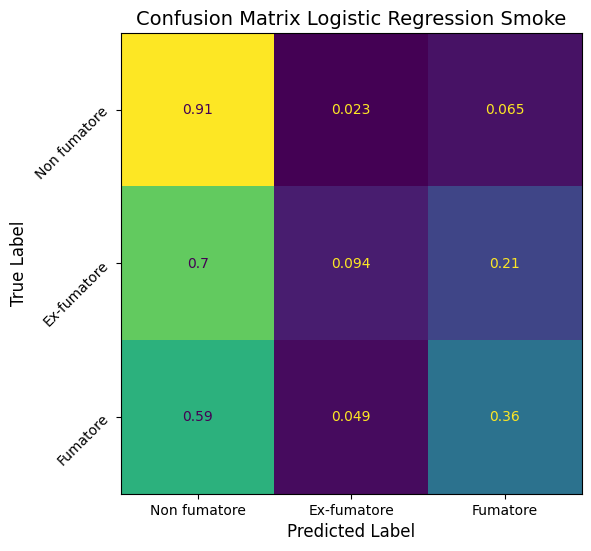
\includegraphics[width=\columnwidth,height=0.75\columnwidth,keepaspectratio]{screen_results/confusion_matrix_first_example_s.png}
\end{minipage}
\end{center}

\subsection*{Drink}
\begin{center}
\begin{minipage}[c]{0.50\columnwidth}
\resizebox{\columnwidth}{!}{%
\begin{tabular}{lcccc}
\toprule
Label  & Precision & Recall & F1-score & Support \\
\midrule
Y      & 0.70      & 0.70   & 0.70     & 135539 \\
N      & 0.71      & 0.70   & 0.70     & 137940 \\
\midrule
Accuracy     & --        & --     & 0.70     & 273479 \\
Macro avg    & 0.70      & 0.70   & 0.70     & 273479 \\
Weighted avg & 0.70      & 0.70   & 0.70     & 273479 \\
\bottomrule
\end{tabular}%
}
\end{minipage}\hspace{\columnsep}%
\begin{minipage}[c]{0.40\columnwidth}
\centering
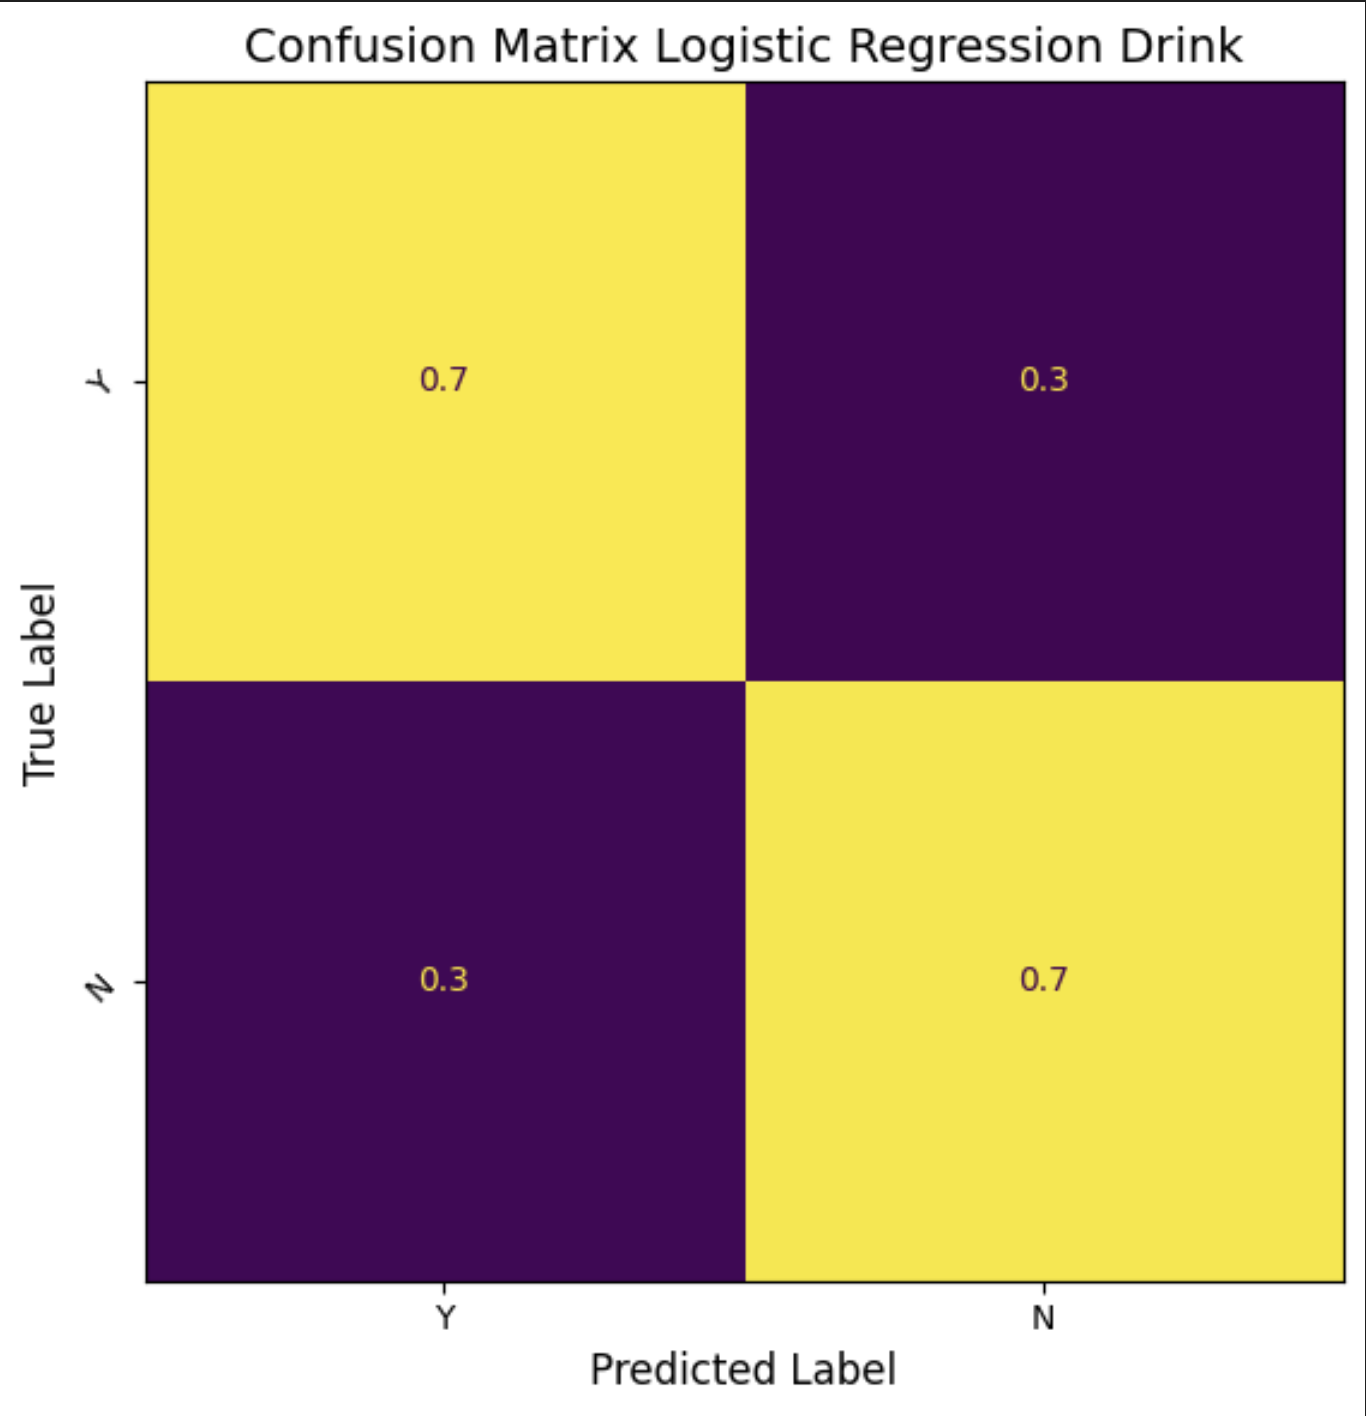
\includegraphics[width=\columnwidth,height=0.75\columnwidth,keepaspectratio]{screen_results/confusion_matrix_first_example_d.png}
\end{minipage}
\end{center}

%%%%%%%%%%%%%%%%%%%%%%%%%%%%%%%%%%%%%%%%%%%%%%%%%%%%%%%%%%%%%%%%%%%%%%%%%%%%%%
% Random Forest
%%%%%%%%%%%%%%%%%%%%%%%%%%%%%%%%%%%%%%%%%%%%%%%%%%%%%%%%%%%%%%%%%%%%%%%%%%%%%%

\subsection{Random Forest}

Di seguito verranno invece riportati i risultati per quanto riguarda quello che abbiamo categorizzato come il miglior modello tra tutti quelli testati: la Random Forest; come si potrà evincere infatti, oltre ad avere la F1-score e l'accuratezza tra le più alte tra tutti i modelli testati, è anche il modello che riesce meglio a separare la classe dei "Non fumatori" dalla classe combinata "Fumatori e Ex-fumatori" e a sua volta è anche la migliore che riesce a separare queste ultime due (anche se comunque non in maniera ottimale).
Per di più, proprio grazie a questi risultati ottenuti dalla Random Forest abbiamo avuto l'idea di testare un classificatore di tipo gerarchico, dunque si è rivelato un modello fondamentale per il nostro progetto.

\paragraph{Cross validation}
Siccome la Random Forest si è rivelato il modello migliore in assoluto, abbiamo anche pensato di fare cross-validation per valutare in maniera più precisa le performance del modello; siccome nello step della feature selection abbiamo allenato il nostro modello tenendo però costante il set di train e di validazione, potremmo aver "overfittato" in base alla suddivisione specifica, quindi con la cross-validation, abbiamo testato il modello su diverse porzioni del dataset per poter valutare in maniera esaustiva il modello. Specifichiamo che avremmo potuto effettuare la cross-validation anche per tutti gli altri modelli, ma vista la quantità di modelli testati ed il tempo necessario per compiere cross-validation ci siamo limitati a farla solo per il modello migliore tra tutti quelli testati.

\subsection*{Smoke (Modello Base)}
\begin{center}
\begin{minipage}[c]{0.50\columnwidth}
\resizebox{\columnwidth}{!}{%
\begin{tabular}{lcccc}
\toprule
Label        & Precision & Recall & F1-score & Support \\
\midrule
Non-smoker   & 0.82      & 0.84   & 0.83     & 167528 \\
Ex-smoker    & 0.44      & 0.35   & 0.39     & 47377  \\
Smoker       & 0.51      & 0.56   & 0.54     & 58574  \\
\midrule
Accuracy     & --        & --     & 0.69     & 273479 \\
Macro avg    & 0.59      & 0.58   & 0.58     & 273479 \\
Weighted avg & 0.69      & 0.69   & 0.69     & 273479 \\
\bottomrule
\end{tabular}%
}
\end{minipage}\hspace{\columnsep}%
\begin{minipage}[c]{0.40\columnwidth}
\centering
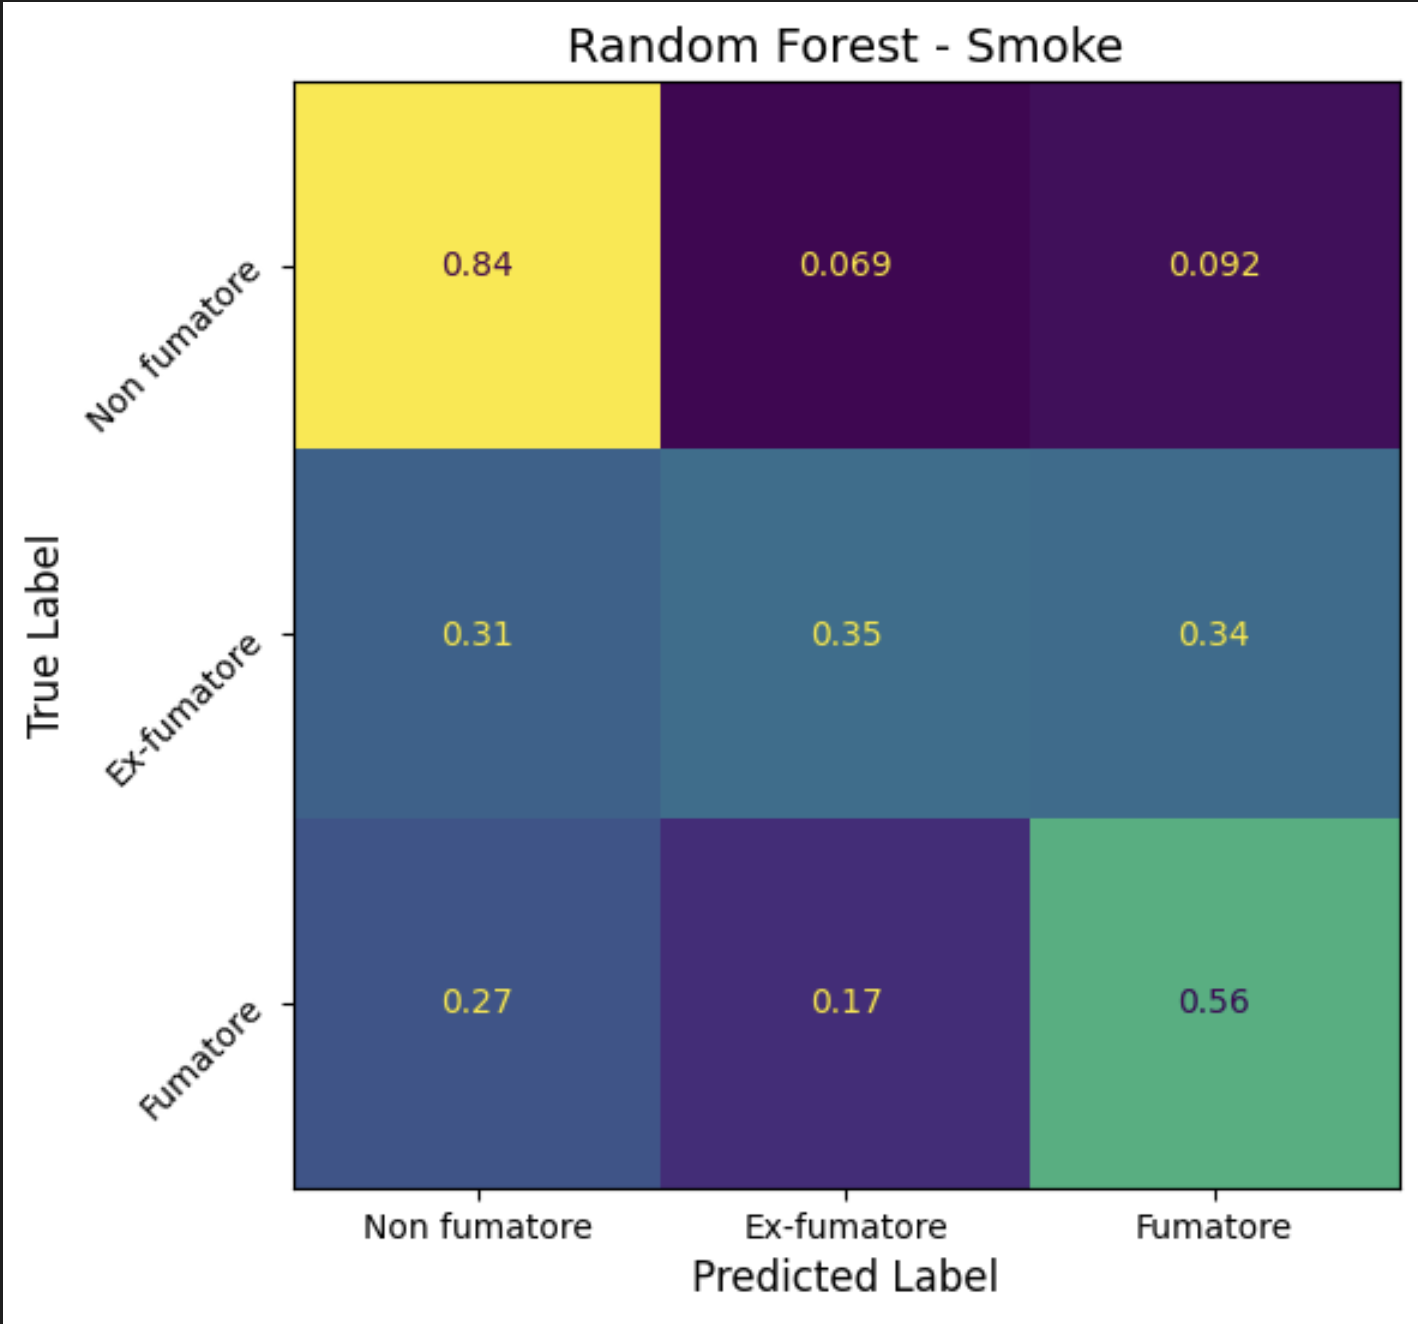
\includegraphics[width=\columnwidth,height=0.75\columnwidth,keepaspectratio]{screen_results/confusion_matrix_rf_base_s.png}
\end{minipage}
\end{center}

\subsection*{Drink (Modello Base)}
\begin{center}
\begin{minipage}[c]{0.50\columnwidth}
\resizebox{\columnwidth}{!}{%
\begin{tabular}{lcccc}
\toprule
Label  & Precision & Recall & F1-score & Support \\
\midrule
Y      & 0.72      & 0.71   & 0.72     & 135539 \\
N      & 0.72      & 0.73   & 0.73     & 137940 \\
\midrule
Accuracy     & --        & --     & 0.72     & 273479 \\
Macro avg    & 0.72      & 0.72   & 0.72     & 273479 \\
Weighted avg & 0.72      & 0.72   & 0.72     & 273479 \\
\bottomrule
\end{tabular}%
}
\end{minipage}\hspace{\columnsep}%
\begin{minipage}[c]{0.40\columnwidth}
\centering
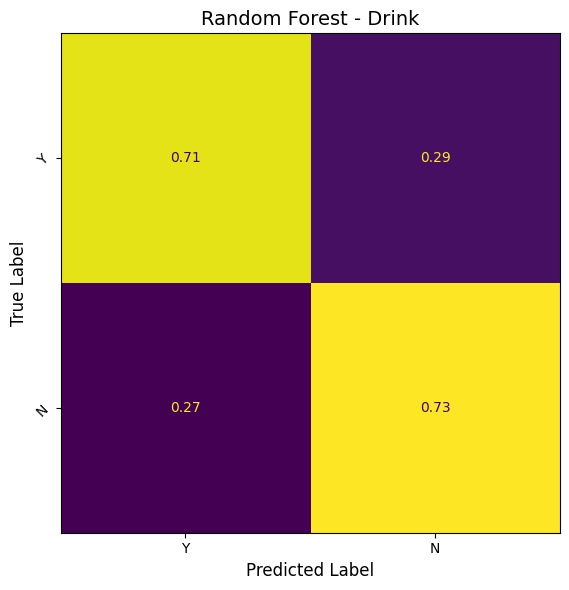
\includegraphics[width=\columnwidth,height=0.75\columnwidth,keepaspectratio]{screen_results/confusion_matrix_rf_base_d.png}
\end{minipage}
\end{center}

\label{bestmodel_smoke}
\subsection*{Smoke (Modello Ottimizzato)}
\begin{center}
\begin{minipage}[c]{0.50\columnwidth}
\resizebox{\columnwidth}{!}{%
\begin{tabular}{lcccc}
\toprule
Label        & Precision & Recall & F1-score & Support \\
\midrule
Non-smoker   & 0.94      & 0.73   & 0.82     & 179990 \\
Ex-smoker    & 0.41      & 0.58   & 0.48     & 52103  \\
Smoker       & 0.49      & 0.64   & 0.55     & 63429  \\
\midrule
Accuracy     & --        & --     & 0.68     & 295522 \\
Macro avg    & 0.61      & 0.65   & 0.62     & 295522 \\
Weighted avg & 0.75      & 0.68   & 0.70     & 295522 \\
\bottomrule
\end{tabular}%
}
\end{minipage}\hspace{\columnsep}%
\begin{minipage}[c]{0.40\columnwidth}
\centering
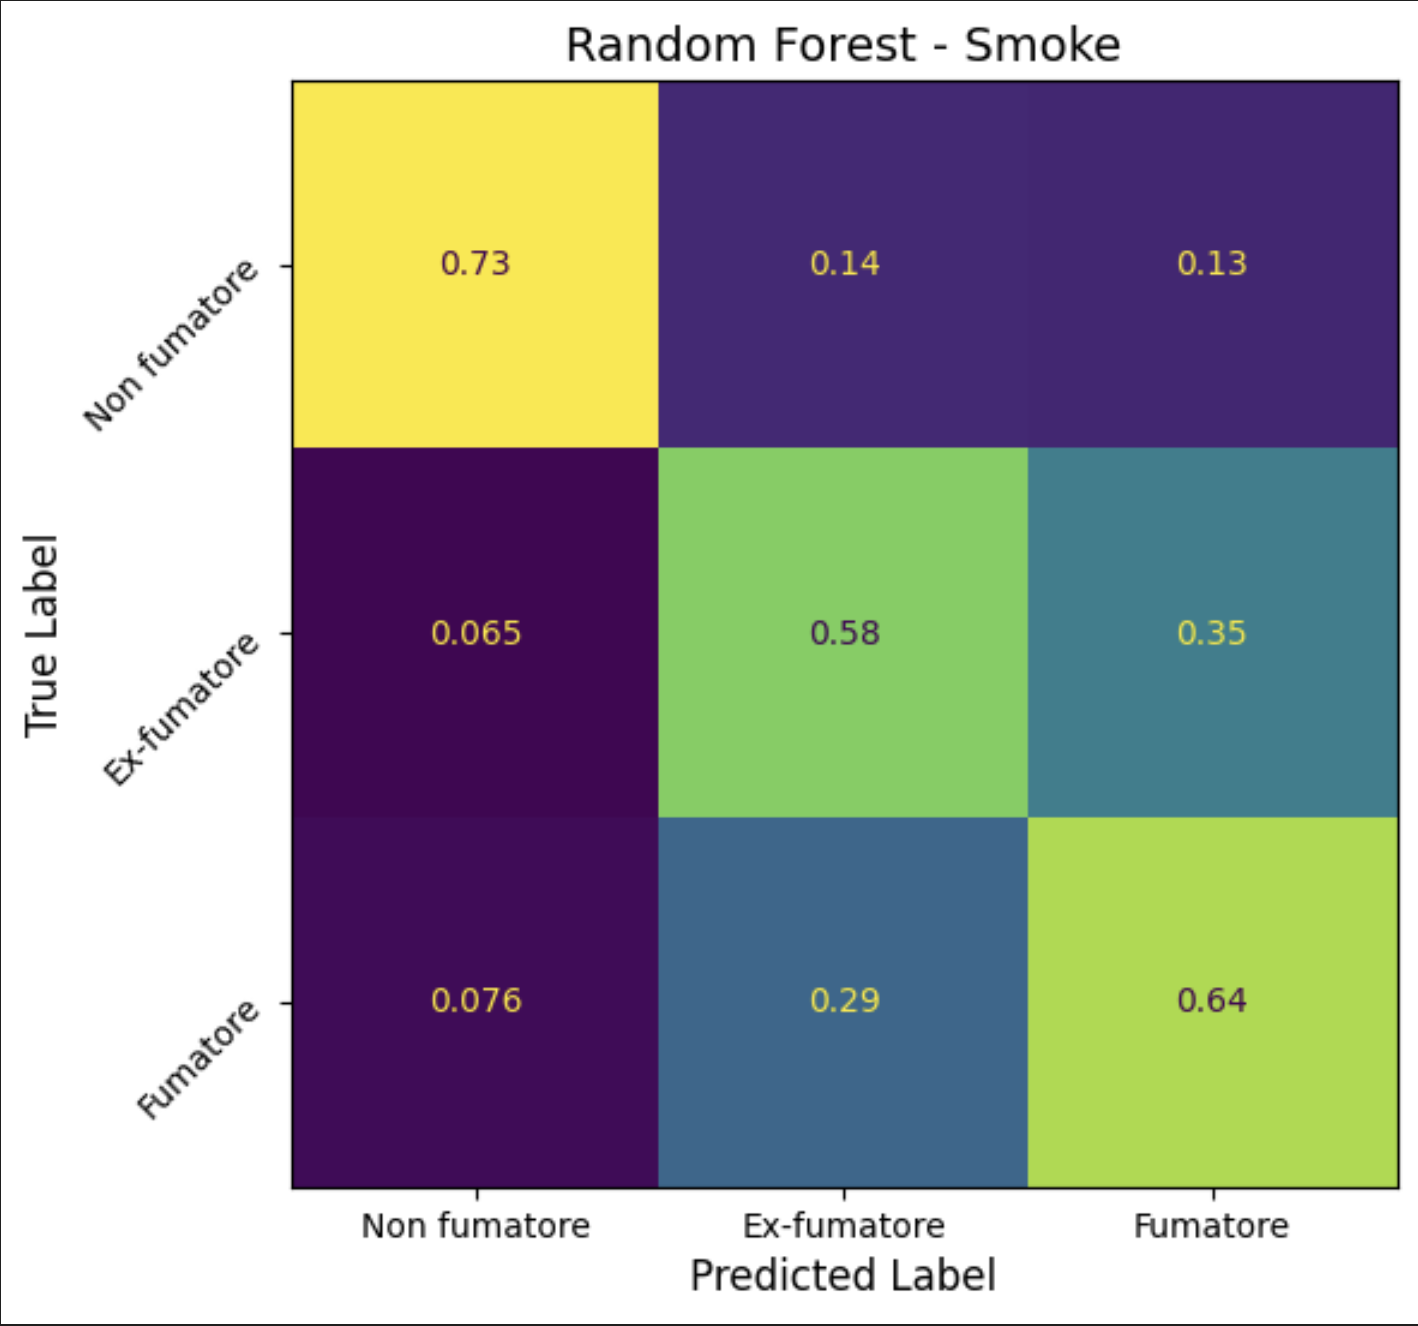
\includegraphics[width=\columnwidth,height=0.75\columnwidth,keepaspectratio]{screen_results/confusion_matrix_rf_optimized_s.png}
\end{minipage}
\end{center}

\label{bestmodel_drink}
\subsection*{Drink (Modello Ottimizzato)}
\begin{center}
\begin{minipage}[c]{0.50\columnwidth}
\resizebox{\columnwidth}{!}{%
\begin{tabular}{lcccc}
\toprule
Label  & Precision & Recall & F1-score & Support \\
\midrule
Y      & 0.74      & 0.71   & 0.73     & 147869 \\
N      & 0.72      & 0.75   & 0.74     & 147653 \\
\midrule
Accuracy     & --        & --     & 0.73     & 295522 \\
Macro avg    & 0.73      & 0.73   & 0.73     & 295522 \\
Weighted avg & 0.73      & 0.73   & 0.73     & 295522 \\
\bottomrule
\end{tabular}%
}
\end{minipage}\hspace{\columnsep}%
\begin{minipage}[c]{0.40\columnwidth}
\centering
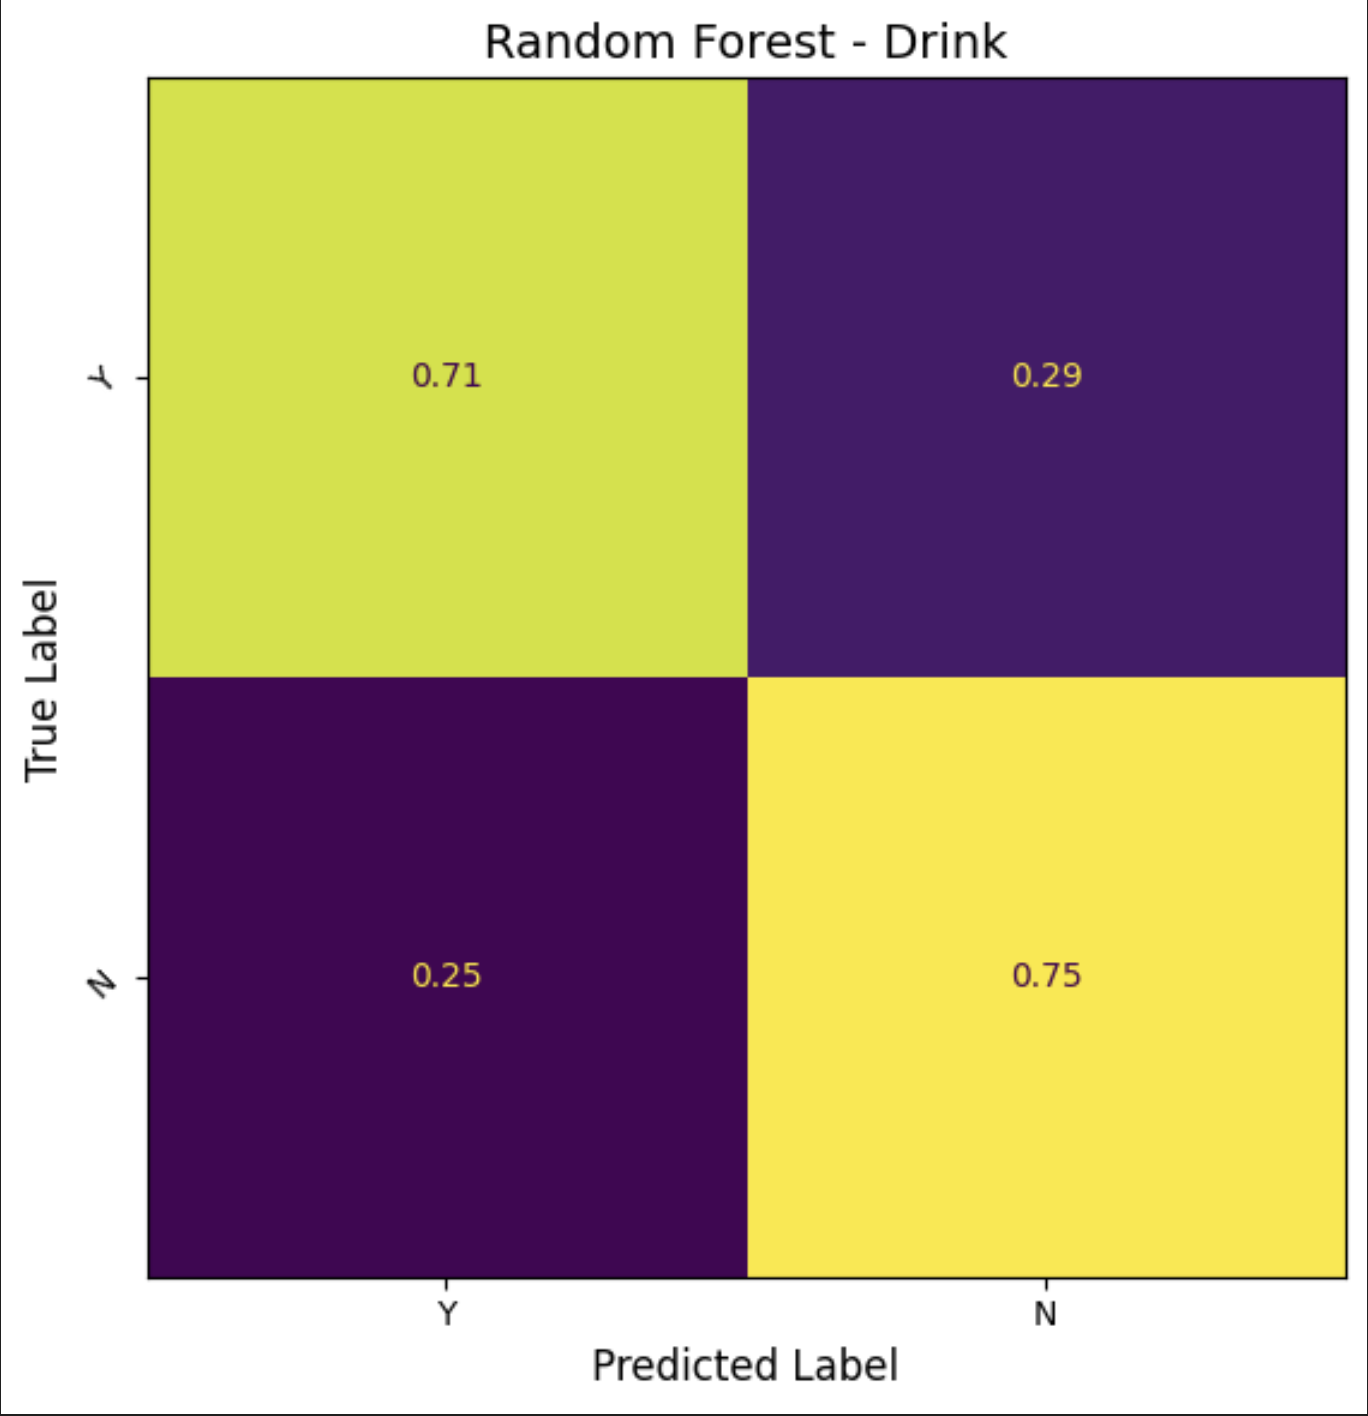
\includegraphics[width=\columnwidth,height=0.75\columnwidth,keepaspectratio]{screen_results/confusion_matrix_rf_optimized_d.png}
\end{minipage}
\end{center}

%%%%%%%%%%%%%%%%%%%%%%%%%%%%%%%%%%%%%%%%%%%%%%%%%%%%%%%%%%%%%%%%%%%%%%%%%%%%%%
% Altri modelli (SVM lineare, KNN, AdaBoost)
%%%%%%%%%%%%%%%%%%%%%%%%%%%%%%%%%%%%%%%%%%%%%%%%%%%%%%%%%%%%%%%%%%%%%%%%%%%%%%

\subsection{Altri modelli (SVM lineare, KNN, AdaBoost)}

Per poter confrontare i risultati della Random Forest con tutti gli altri modelli testati, riportiamo anche i risultati di questi appena citati; come si potrà evincere, qualche modello (come SVM) si avvicina molto alle performance della Random Forest ma risulta comunque leggermente peggiore, mentre per altri modelli si noterà marcatamente la differenza non tanto di metriche come la F1-score quanto della capacità di classificare i sample appartenenti agli "Ex-fumatori" e "Fumatori".
Purtroppo per quanto riguarda la classificazione riguardante il consumo di alcool, da adesso in poi rimarrà praticamente la medesima.

\subsection*{AdaBoost (Smoke)}
\begin{center}
\begin{minipage}[c]{0.50\columnwidth}
\resizebox{\columnwidth}{!}{%
\begin{tabular}{lcccc}
\toprule
Label        & Precision & Recall & F1-score & Support \\
\midrule
Non-smoker   & 0.83      & 0.83   & 0.83     & 119747 \\
Ex-smoker    & 0.45      & 0.32   & 0.37     & 34738  \\
Smoker       & 0.50      & 0.63   & 0.56     & 42530  \\
\midrule
Accuracy     & --        & --     & 0.70     & 197015 \\
Macro avg    & 0.59      & 0.59   & 0.59     & 197015 \\
Weighted avg & 0.69      & 0.70   & 0.69     & 197015 \\
\bottomrule
\end{tabular}%
}
\end{minipage}\hspace{\columnsep}%
\begin{minipage}[c]{0.40\columnwidth}
\centering
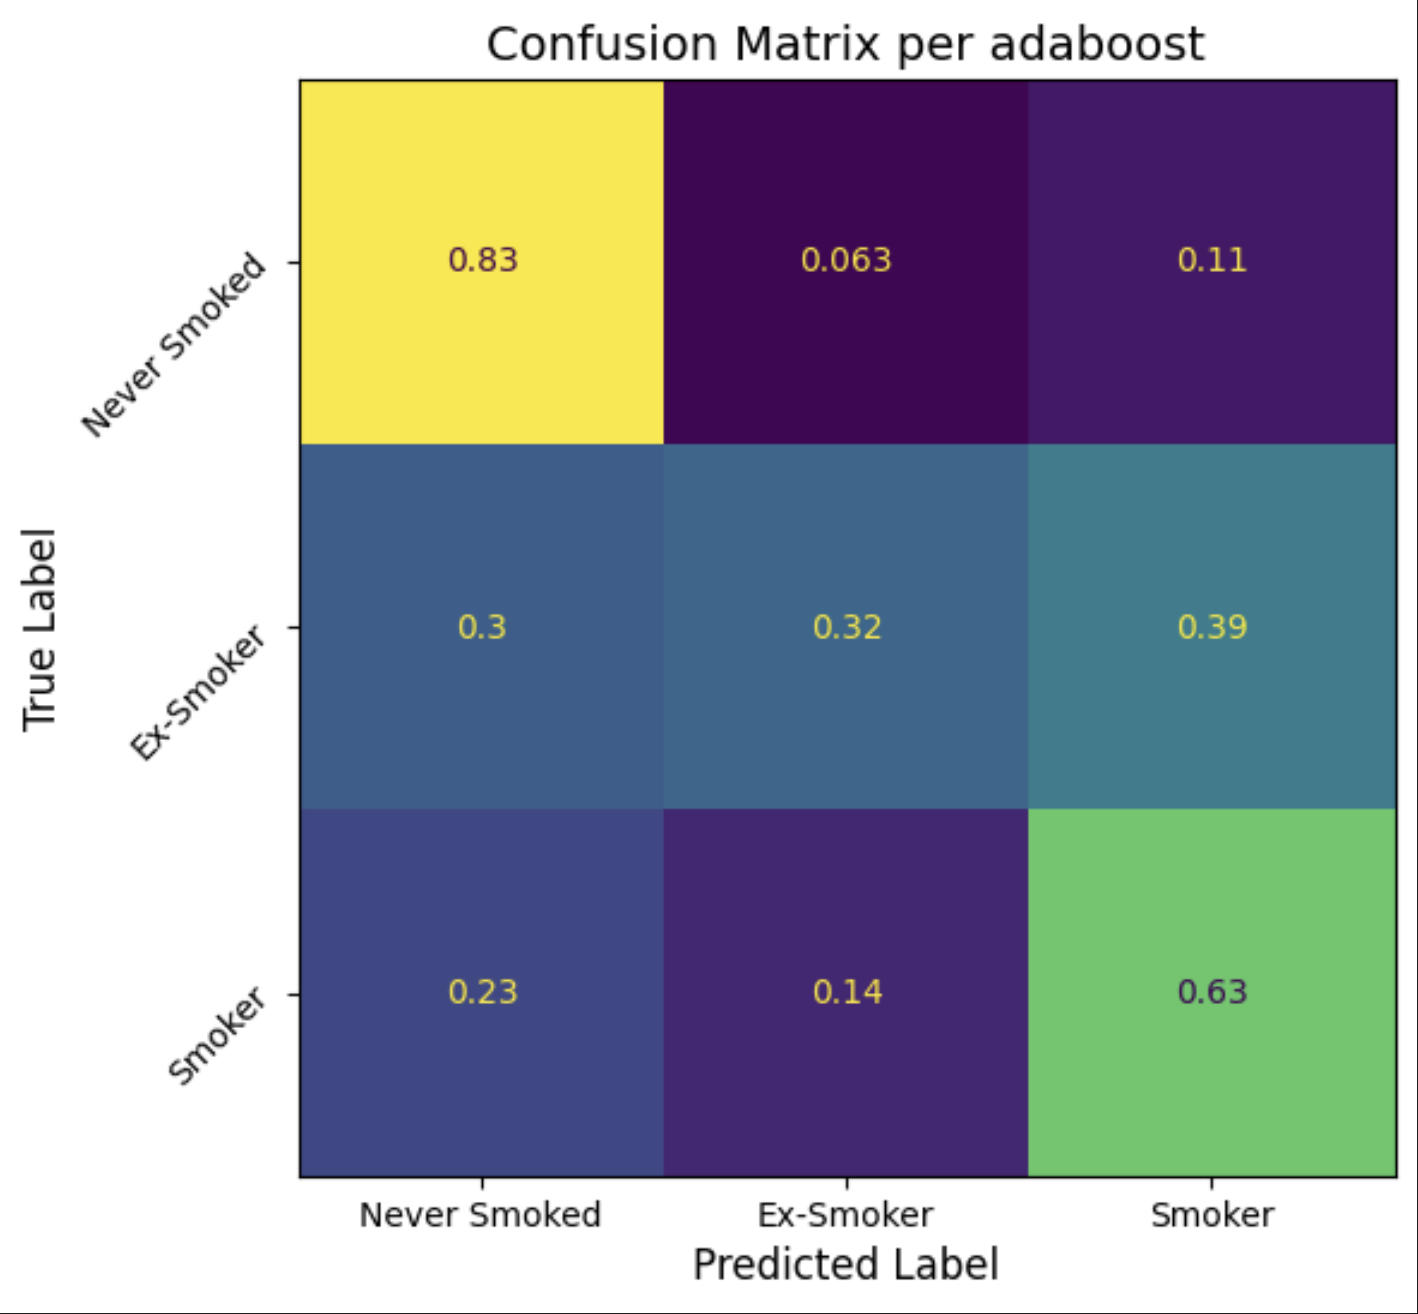
\includegraphics[width=\columnwidth,height=0.75\columnwidth,keepaspectratio]{screen_results/confusion_matrix_adaboost_s.png}
\end{minipage}
\end{center}

\subsection*{SVM (Smoke)}
\begin{center}
\begin{minipage}[c]{0.50\columnwidth}
\resizebox{\columnwidth}{!}{%
\begin{tabular}{lcccc}
\toprule
Label        & Precision & Recall & F1-score & Support \\
\midrule
Non-smoker   & 0.94      & 0.73   & 0.82     & 119747 \\
Ex-smoker    & 0.41      & 0.55   & 0.47     & 34738  \\
Smoker       & 0.47      & 0.65   & 0.55     & 42530  \\
\midrule
Accuracy     & --        & --     & 0.68     & 197015 \\
Macro avg    & 0.61      & 0.64   & 0.61     & 197015 \\
Weighted avg & 0.75      & 0.68   & 0.70     & 197015 \\
\bottomrule
\end{tabular}%
}
\end{minipage}\hspace{\columnsep}%
\begin{minipage}[c]{0.40\columnwidth}
\centering
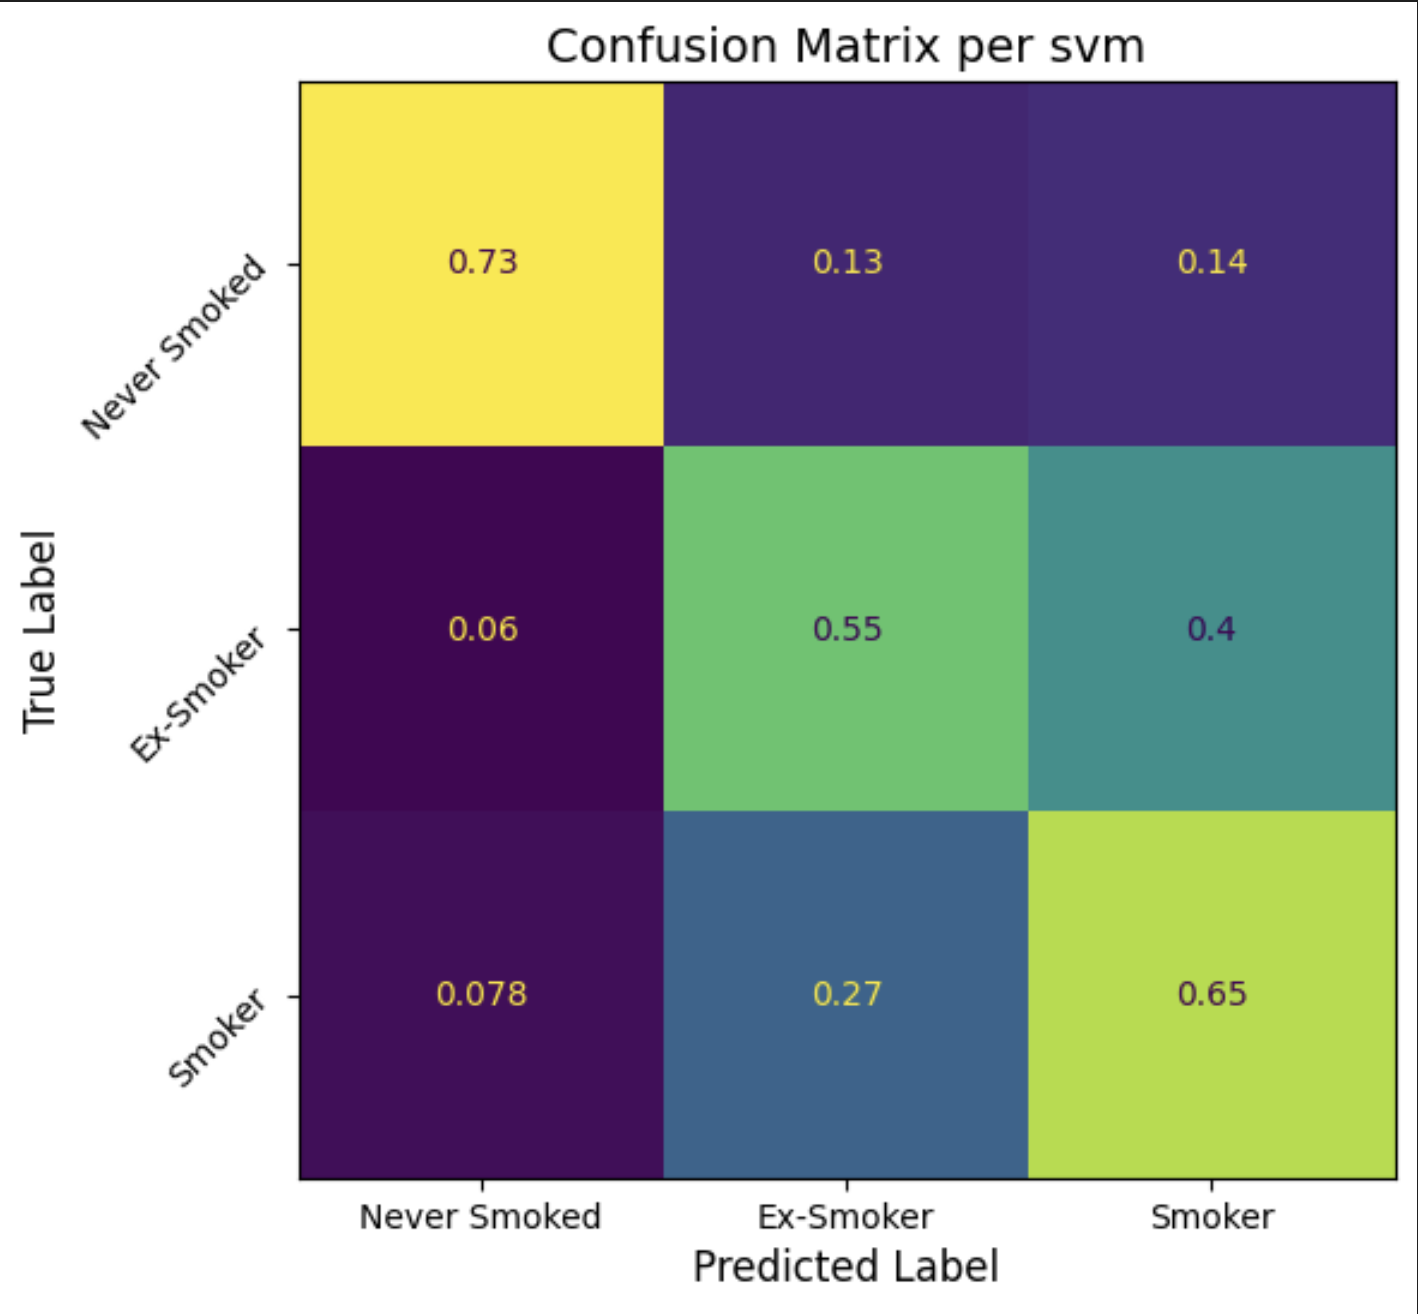
\includegraphics[width=\columnwidth,height=0.75\columnwidth,keepaspectratio]{screen_results/confusion_matrix_svm_s.png}
\end{minipage}
\end{center}

\subsection*{KNN (Smoke)}
\begin{center}
\begin{minipage}[c]{0.50\columnwidth}
\resizebox{\columnwidth}{!}{%
\begin{tabular}{lcccc}
\toprule
Label        & Precision & Recall & F1-score & Support \\
\midrule
Non-smoker   & 0.85      & 0.80   & 0.83     & 119747 \\
Ex-smoker    & 0.44      & 0.43   & 0.43     & 34738  \\
Smoker       & 0.49      & 0.59   & 0.54     & 42530  \\
\midrule
Accuracy     & --        & --     & 0.69     & 197015 \\
Macro avg    & 0.60      & 0.61   & 0.60     & 197015 \\
Weighted avg & 0.70      & 0.69   & 0.70     & 197015 \\
\bottomrule
\end{tabular}%
}
\end{minipage}\hspace{\columnsep}%
\begin{minipage}[c]{0.40\columnwidth}
\centering
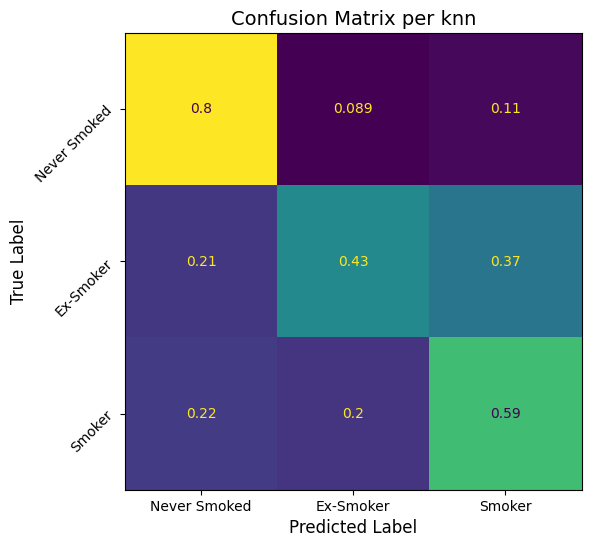
\includegraphics[width=\columnwidth,height=0.75\columnwidth,keepaspectratio]{screen_results/confusion_matrix_knn_s.png}
\end{minipage}
\end{center}

\subsection*{AdaBoost (Drink)}
\begin{center}
\begin{minipage}[c]{0.50\columnwidth}
\resizebox{\columnwidth}{!}{%
\begin{tabular}{lcccc}
\toprule
Label & Precision & Recall & F1-score & Support \\
\midrule
Y     & 0.73      & 0.73   & 0.73     & 98396 \\
N     & 0.73      & 0.73   & 0.73     & 98619 \\
\midrule
Accuracy     & --        & --     & 0.73     & 197015 \\
Macro avg    & 0.73      & 0.73   & 0.73     & 197015 \\
Weighted avg & 0.73      & 0.73   & 0.73     & 197015 \\
\bottomrule
\end{tabular}%
}
\end{minipage}\hspace{\columnsep}%
\begin{minipage}[c]{0.40\columnwidth}
\centering
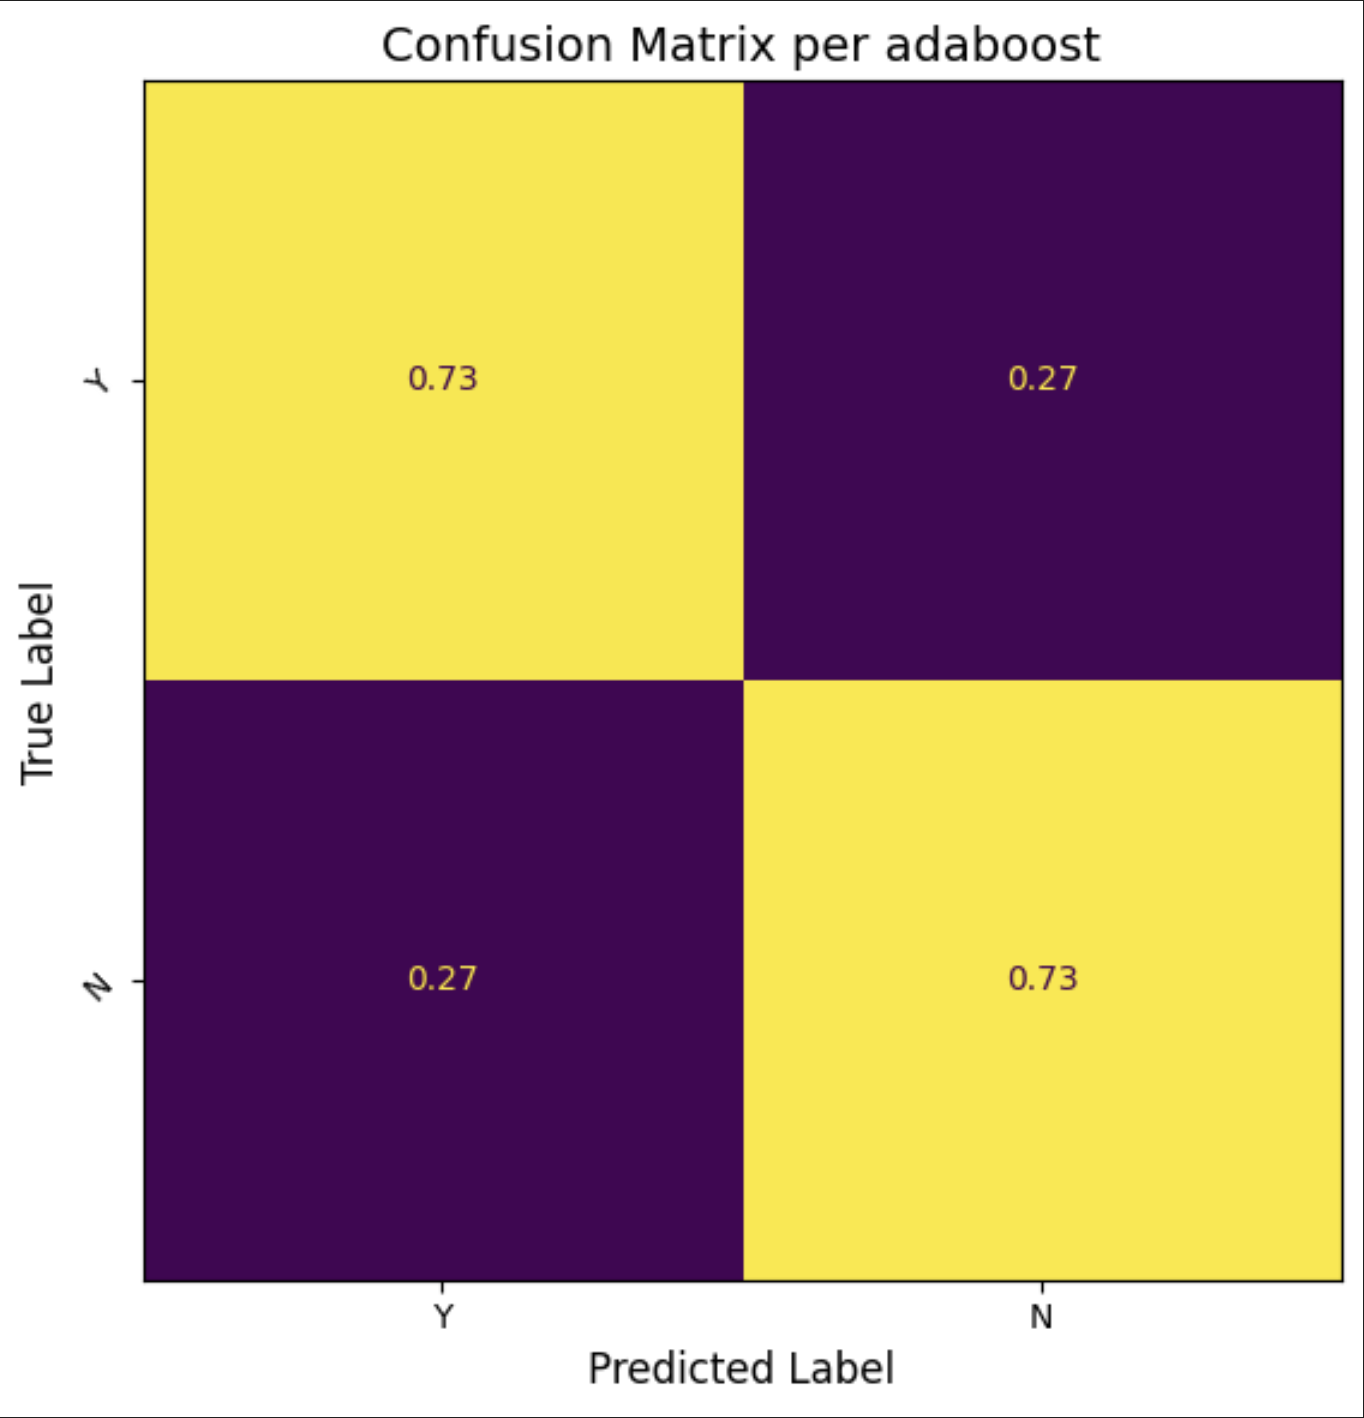
\includegraphics[width=\columnwidth,height=0.75\columnwidth,keepaspectratio]{screen_results/confusion_matrix_adaboost_d.png}
\end{minipage}
\end{center}

\subsection*{SVM (Drink)}
\begin{center}
\begin{minipage}[c]{0.50\columnwidth}
\resizebox{\columnwidth}{!}{%
\begin{tabular}{lcccc}
\toprule
Label & Precision & Recall & F1-score & Support \\
\midrule
Y     & 0.72      & 0.72   & 0.72     & 98396 \\
N     & 0.72      & 0.72   & 0.72     & 98619 \\
\midrule
Accuracy     & --        & --     & 0.72     & 197015 \\
Macro avg    & 0.72      & 0.72   & 0.72     & 197015 \\
Weighted avg & 0.72      & 0.72   & 0.72     & 197015 \\
\bottomrule
\end{tabular}%
}
\end{minipage}\hspace{\columnsep}%
\begin{minipage}[c]{0.40\columnwidth}
\centering
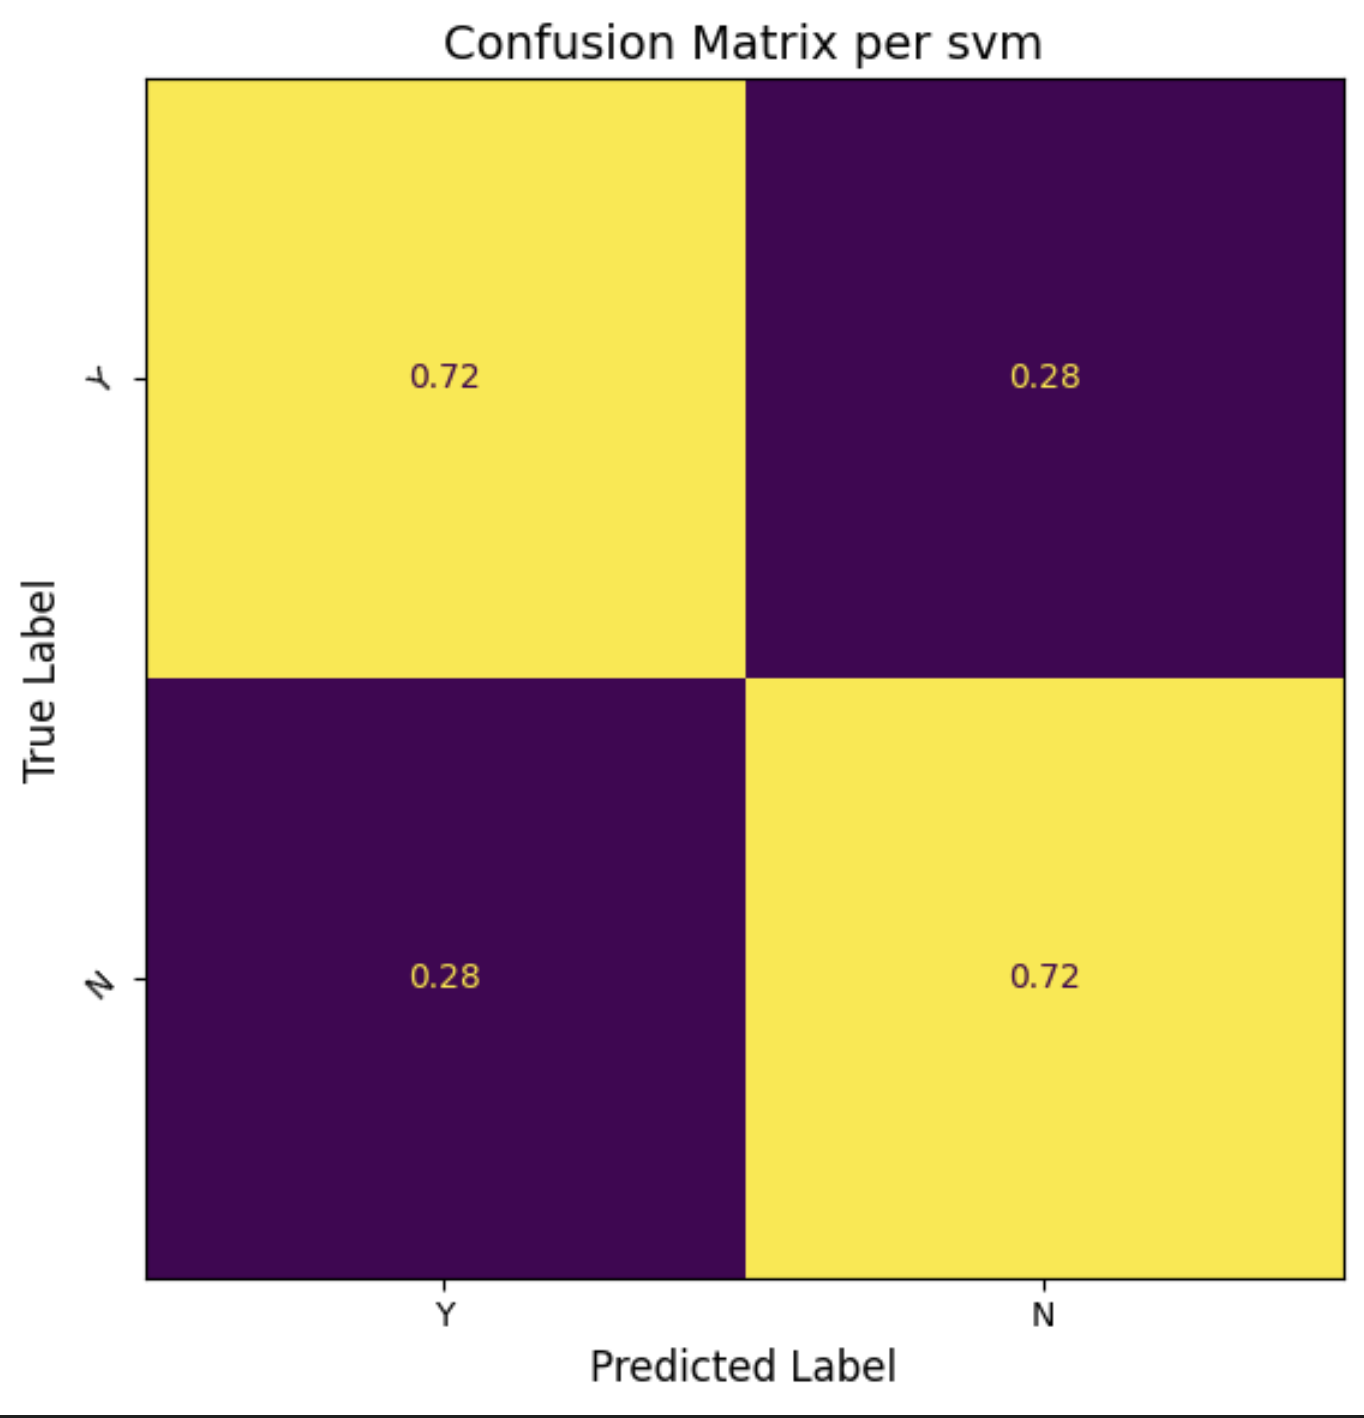
\includegraphics[width=\columnwidth,height=0.75\columnwidth,keepaspectratio]{screen_results/confusion_matrix_svm_d.png}
\end{minipage}
\end{center}

\subsection*{KNN (Drink)}
\begin{center}
\begin{minipage}[c]{0.50\columnwidth}
\resizebox{\columnwidth}{!}{%
\begin{tabular}{lcccc}
\toprule
Label & Precision & Recall & F1-score & Support \\
\midrule
Y     & 0.73      & 0.67   & 0.70     & 98396 \\
N     & 0.70      & 0.76   & 0.73     & 98619 \\
\midrule
Accuracy     & --        & --     & 0.71     & 197015 \\
Macro avg    & 0.72      & 0.71   & 0.71     & 197015 \\
Weighted avg & 0.72      & 0.71   & 0.71     & 197015 \\
\bottomrule
\end{tabular}%
}
\end{minipage}\hspace{\columnsep}%
\begin{minipage}[c]{0.40\columnwidth}
\centering
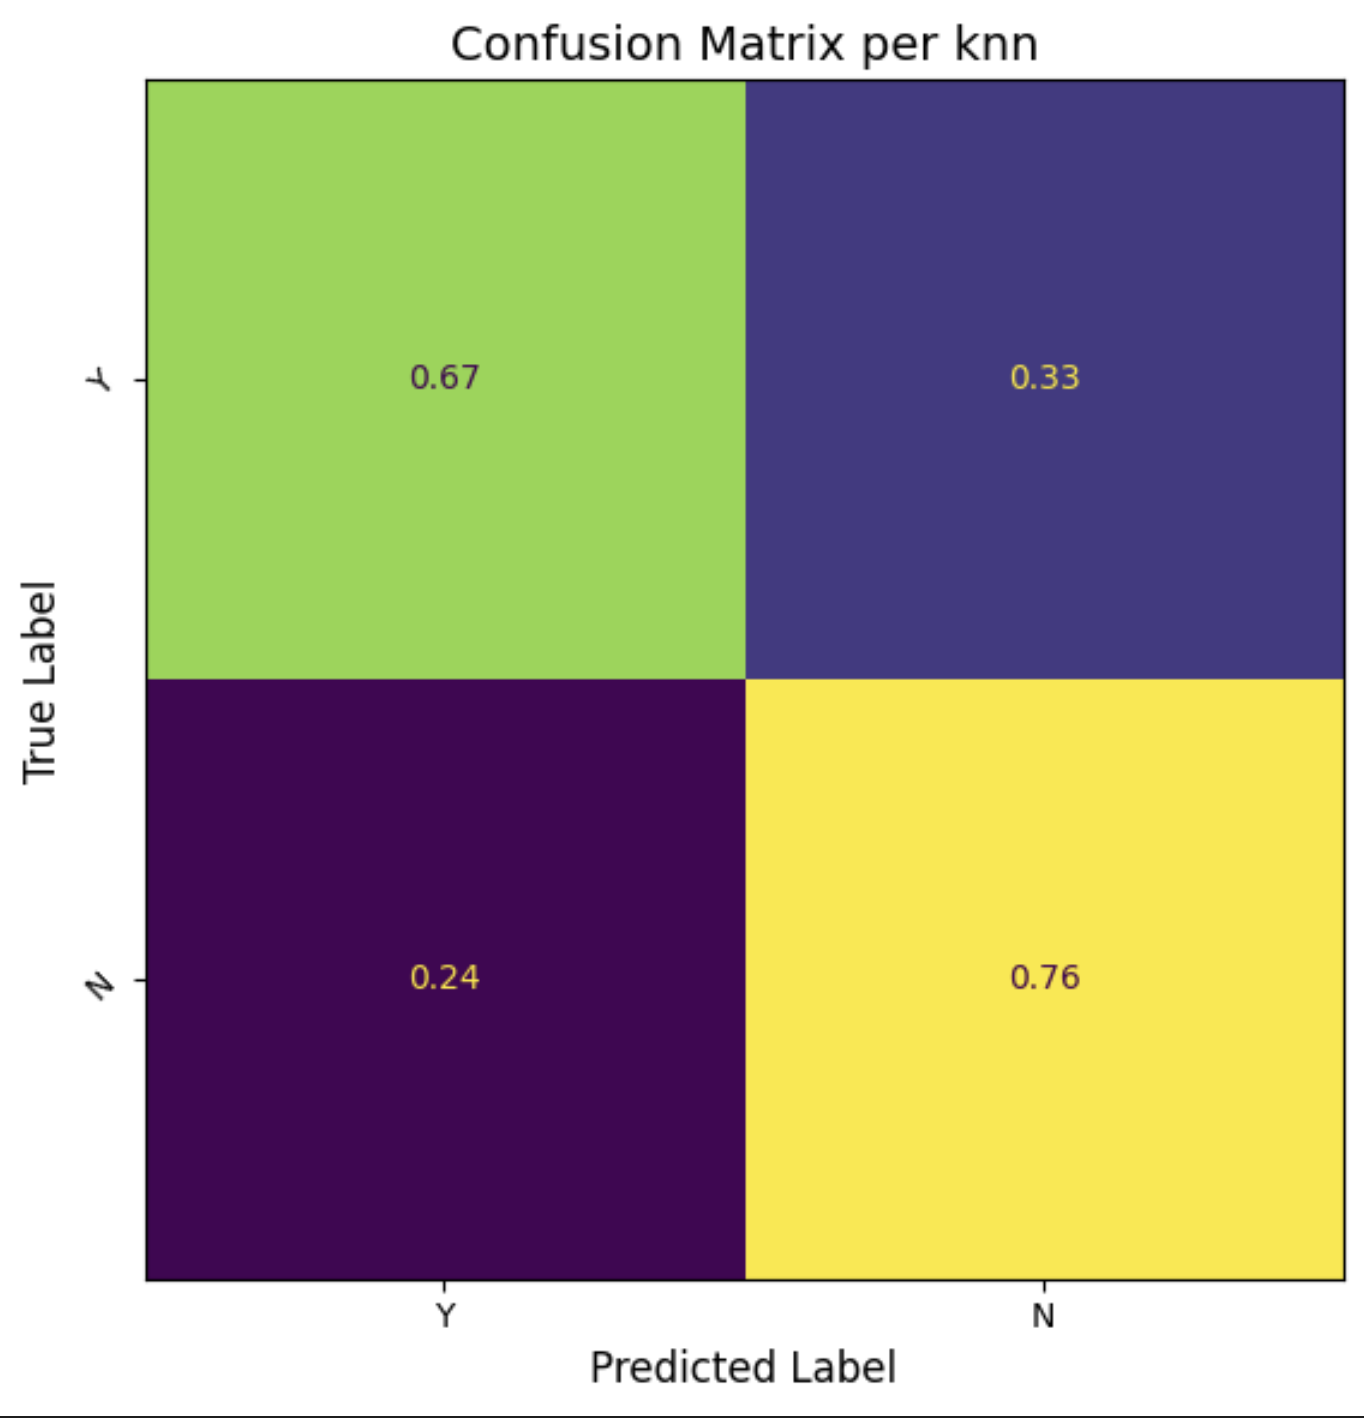
\includegraphics[width=\columnwidth,height=0.75\columnwidth,keepaspectratio]{screen_results/confusion_matrix_knn_d.png}
\end{minipage}
\end{center}

%%%%%%%%%%%%%%%%%%%%%%%%%%%%%%%%%%%%%%%%%%%%%%%%%%%%%%%%%%%%%%%%%%%%%%%%%%%%%%
% Altri modelli con PCA (SVM, KNN)
%%%%%%%%%%%%%%%%%%%%%%%%%%%%%%%%%%%%%%%%%%%%%%%%%%%%%%%%%%%%%%%%%%%%%%%%%%%%%%

\subsection{Altri modelli con PCA (SVM, KNN)}
Come già accennato nella sezione precedente, abbiamo anche testato l'utilizzo della PCA per quanto riguarda i modelli KNN e SVM; purtroppo i risultati non hanno portato a dei miglioramenti.

\subsection*{SVM (Smoke) }
\begin{center}
\begin{minipage}[c]{0.50\columnwidth}
\resizebox{\columnwidth}{!}{%
\begin{tabular}{lcccc}
\toprule
Label        & Precision & Recall & F1-score & Support \\
\midrule
Non-smoker   & 0.89      & 0.76   & 0.82     & 120489 \\
Ex-smoker    & 0.41      & 0.44   & 0.43     & 34990  \\
Smoker       & 0.48      & 0.63   & 0.54     & 42791  \\
\midrule
Accuracy     & --        & --     & 0.68     & 198270 \\
Macro avg    & 0.59      & 0.61   & 0.60     & 198270 \\
Weighted avg & 0.71      & 0.68   & 0.69     & 198270 \\
\bottomrule
\end{tabular}%
}
\end{minipage}\hspace{\columnsep}%
\begin{minipage}[c]{0.40\columnwidth}
\centering
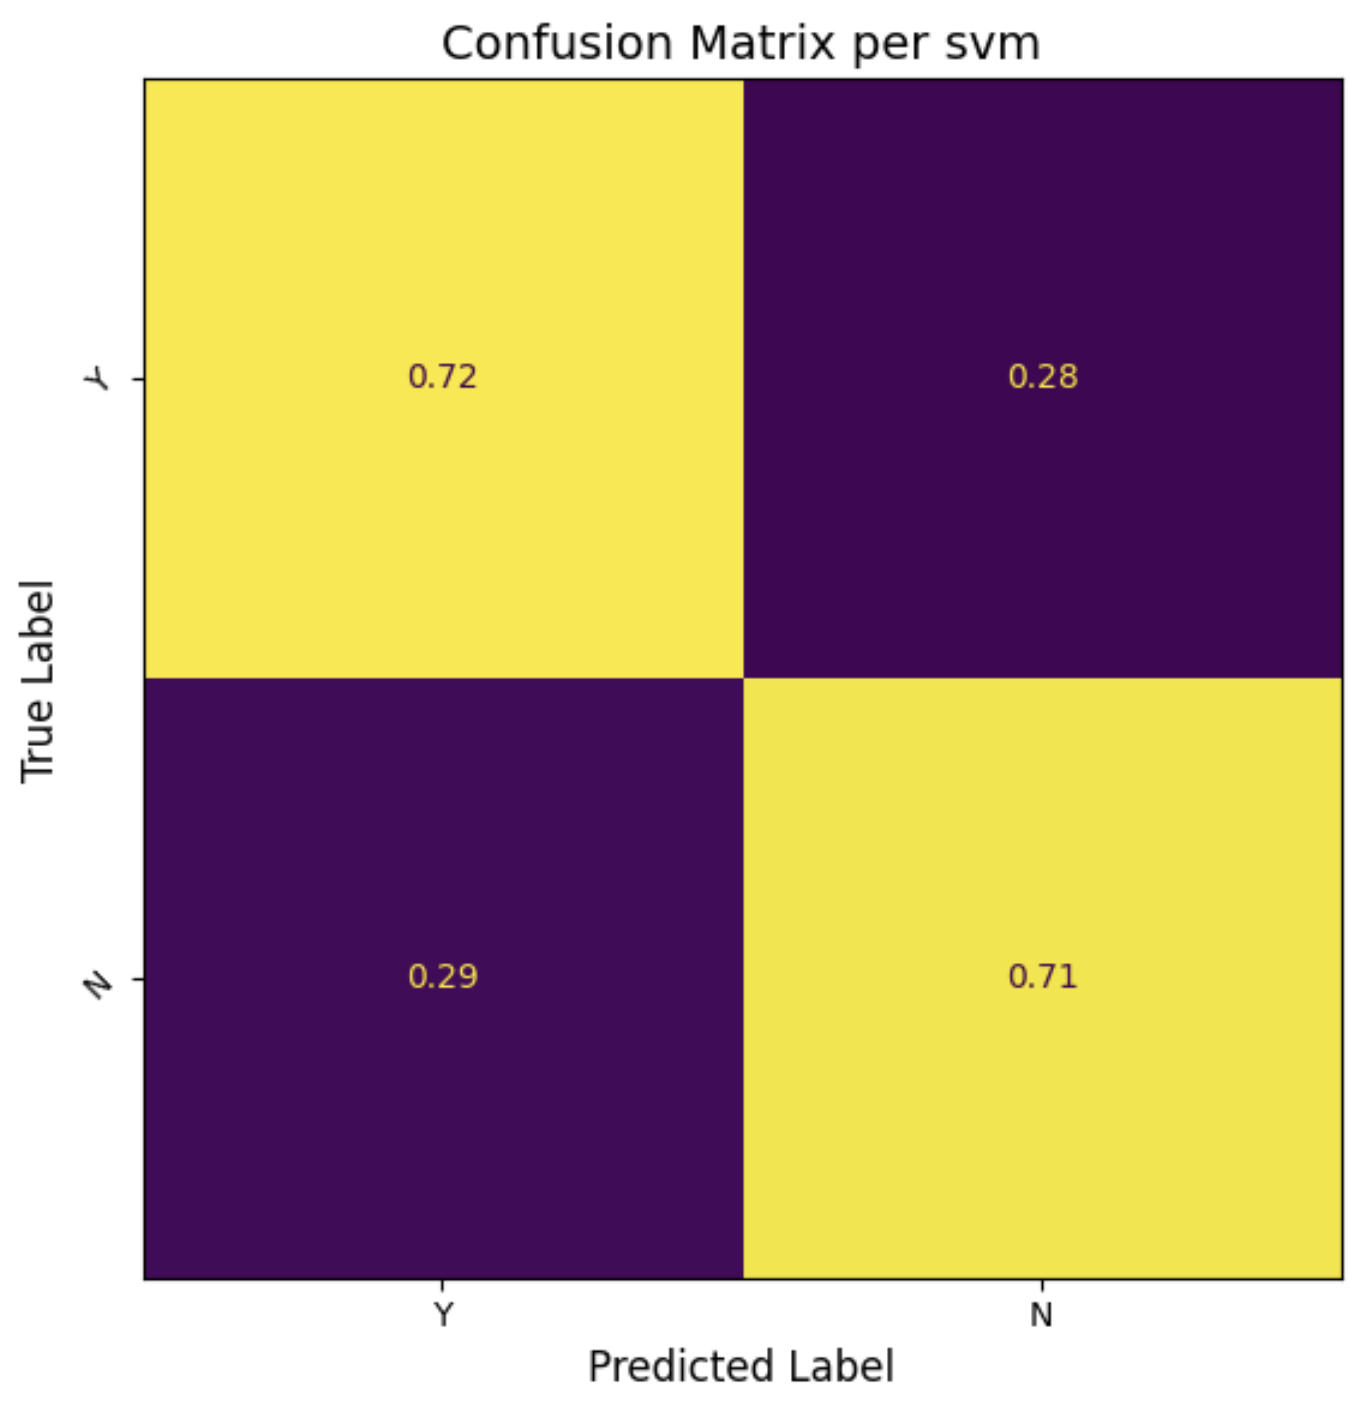
\includegraphics[width=\columnwidth,height=0.75\columnwidth,keepaspectratio]{screen_results/confusion_matrix_svm_pca_d.png} % Adjust image file if needed.
\end{minipage}
\end{center}

\subsection*{KNN (Smoke) }
\begin{center}
\begin{minipage}[c]{0.50\columnwidth}
\resizebox{\columnwidth}{!}{%
\begin{tabular}{lcccc}
\toprule
Label        & Precision & Recall & F1-score & Support \\
\midrule
Non-smoker   & 0.82      & 0.82   & 0.82     & 120489 \\
Ex-smoker    & 0.43      & 0.34   & 0.38     & 34990  \\
Smoker       & 0.49      & 0.57   & 0.53     & 42791  \\
\midrule
Accuracy     & --        & --     & 0.68     & 198270 \\
Macro avg    & 0.58      & 0.58   & 0.58     & 198270 \\
Weighted avg & 0.68      & 0.68   & 0.68     & 198270 \\
\bottomrule
\end{tabular}%
}
\end{minipage}\hspace{\columnsep}%
\begin{minipage}[c]{0.40\columnwidth}
\centering
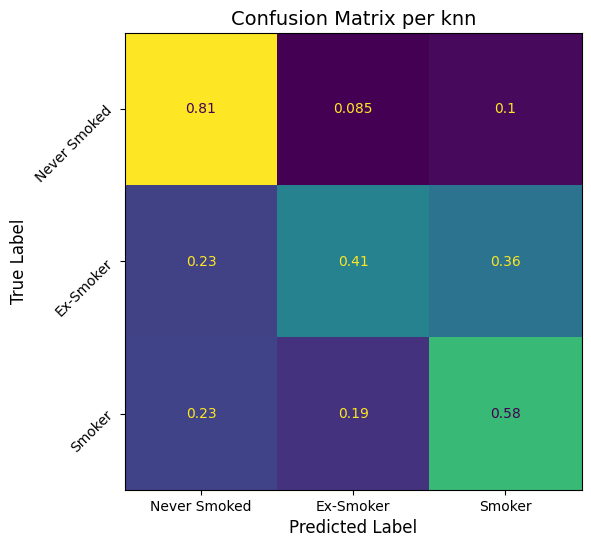
\includegraphics[width=\columnwidth,height=0.75\columnwidth,keepaspectratio]{screen_results/confusion_matrix_knn_pca_s.png}
\end{minipage}
\end{center}

\subsection*{SVM (Drink) }
\begin{center}
\begin{minipage}[c]{0.50\columnwidth}
\resizebox{\columnwidth}{!}{%
\begin{tabular}{lcccc}
\toprule
Label & Precision & Recall & F1-score & Support \\
\midrule
Y     & 0.72      & 0.72   & 0.72     & 99172 \\
N     & 0.72      & 0.72   & 0.72     & 99098 \\
\midrule
Accuracy     & --        & --     & 0.72     & 198270 \\
Macro avg    & 0.72      & 0.72   & 0.72     & 198270 \\
Weighted avg & 0.72      & 0.72   & 0.72     & 198270 \\
\bottomrule
\end{tabular}%
}
\end{minipage}\hspace{\columnsep}%
\begin{minipage}[c]{0.40\columnwidth}
\centering
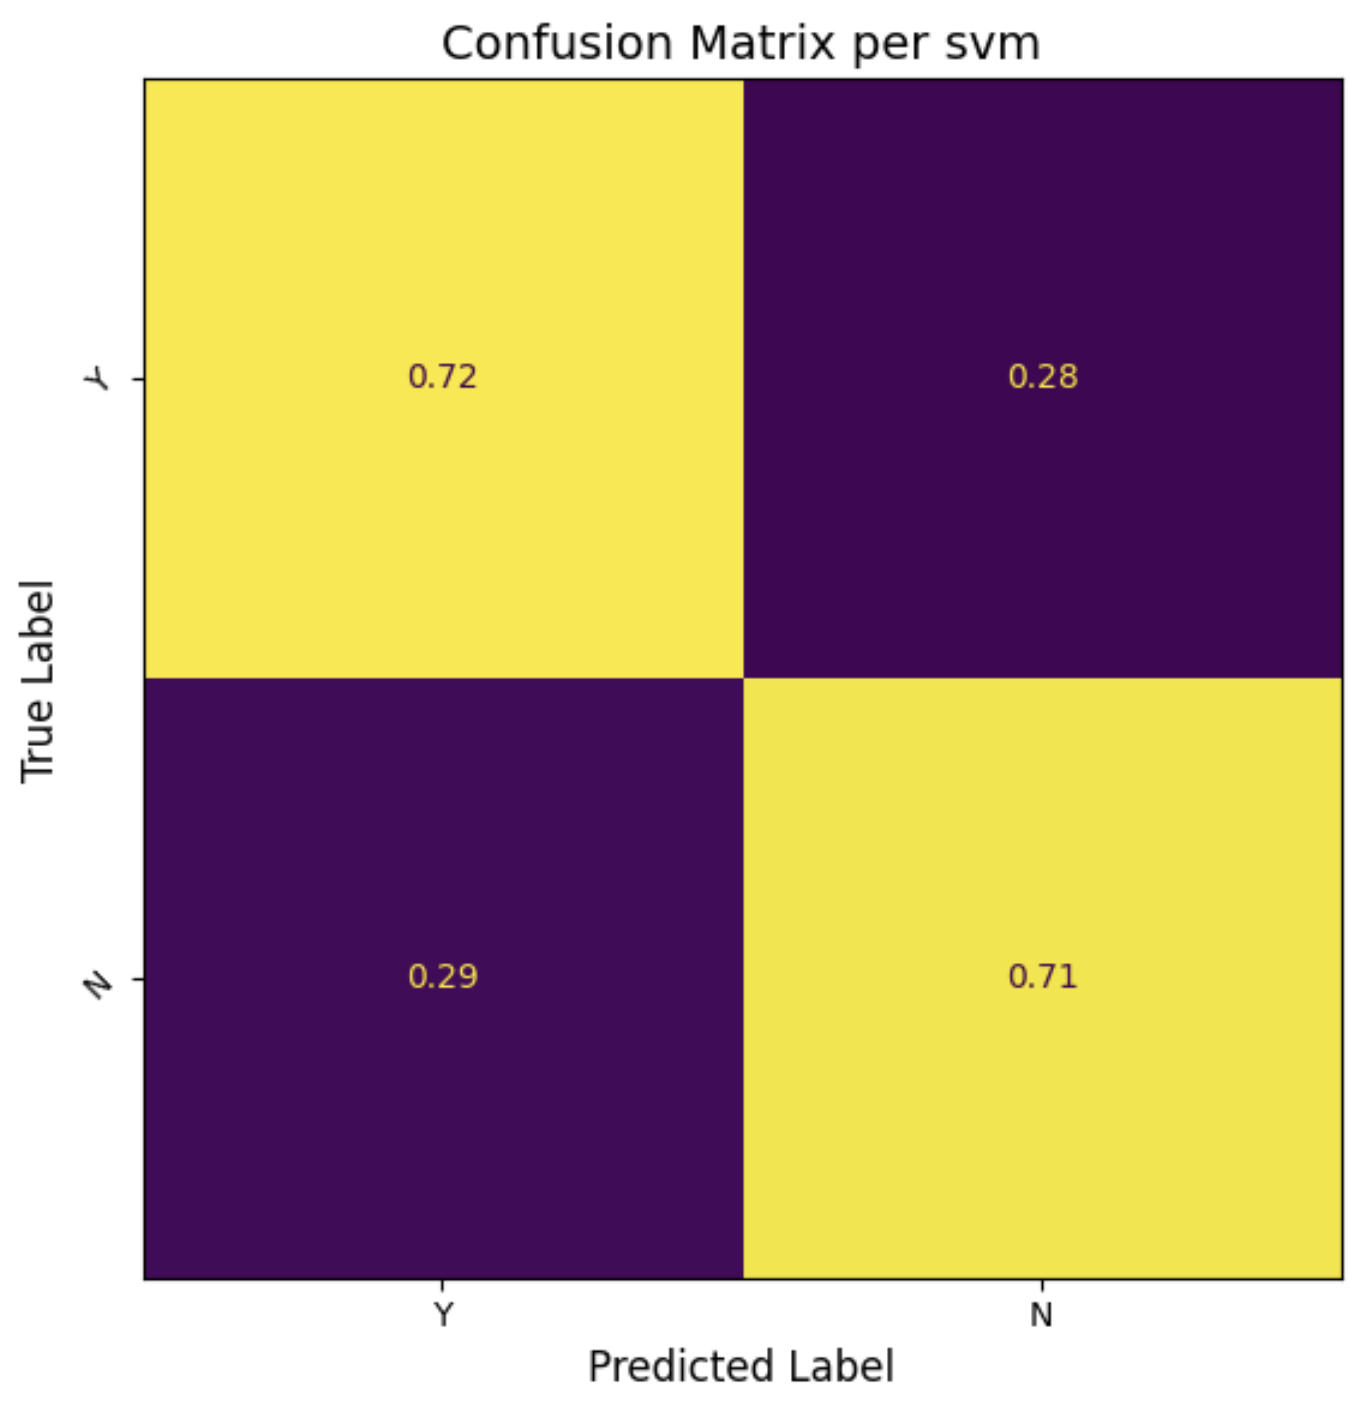
\includegraphics[width=\columnwidth,height=0.75\columnwidth,keepaspectratio]{screen_results/confusion_matrix_svm_pca_d.png}
\end{minipage}
\end{center}

\subsection*{KNN (Drink) }
\begin{center}
\begin{minipage}[c]{0.50\columnwidth}
\resizebox{\columnwidth}{!}{%
\begin{tabular}{lcccc}
\toprule
Label & Precision & Recall & F1-score & Support \\
\midrule
Y     & 0.73      & 0.68   & 0.70     & 99172 \\
N     & 0.70      & 0.75   & 0.72     & 99098 \\
\midrule
Accuracy     & --        & --     & 0.71     & 198270 \\
Macro avg    & 0.71      & 0.71   & 0.71     & 198270 \\
Weighted avg & 0.71      & 0.71   & 0.71     & 198270 \\
\bottomrule
\end{tabular}%
}
\end{minipage}\hspace{\columnsep}%
\begin{minipage}[c]{0.40\columnwidth}
\centering
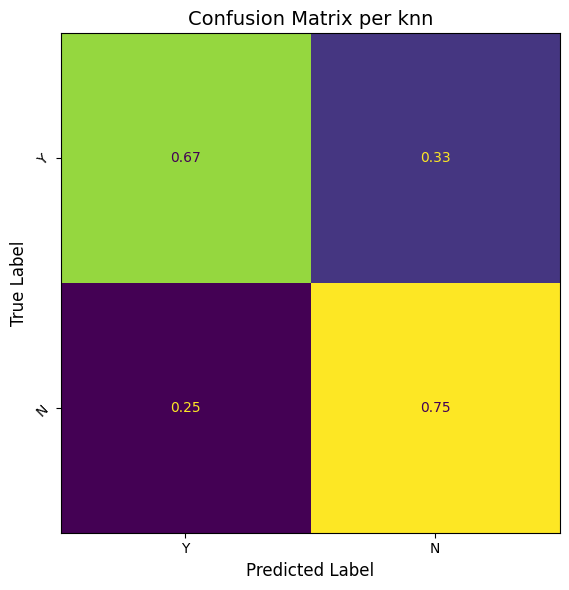
\includegraphics[width=\columnwidth,height=0.75\columnwidth,keepaspectratio]{screen_results/confusion_matrix_knn_pca_d.png}
\end{minipage}
\end{center}

%%%%%%%%%%%%%%%%%%%%%%%%%%%%%%%%%%%%%%%%%%%%%%%%%%%%%%%%%%%%%%%%%%%%%%%%%%%%%%
% Feature Engeneering (Random Forest, AdaBoost, SVM, KNN)
%%%%%%%%%%%%%%%%%%%%%%%%%%%%%%%%%%%%%%%%%%%%%%%%%%%%%%%%%%%%%%%%%%%%%%%%%%%%%%

\subsection{Feature Engeneering (Random Forest, AdaBoost, SVM, KNN)}
Il tentativo di fare feature engeneering, è stato un test che non sapevamo se ed eventualmente in che misura avrebbe influito sui risultati; noi ci siamo limitato ad aggregare le nuove feature ricavate a quelle già esistenti e sicuramente avremmo potuto fare delle prove differenti, per esempio utilizzando solo le nuove feature, oppure facendo feature selection, oppure ancora facendo delle trasformazioni differenti da quelle attuate da noi.
Purtroppo anche in questo caso le performance non sono migliorate rispetto agli step precedenti, però comunque le metriche sono rimaste più o meno invariate, segno che le feature aggiunte non hanno causato overfitting o altri tipi di problemi.

\subsection*{Random Forest (Smoke)}
\begin{center}
\begin{minipage}[c]{0.50\columnwidth}
\resizebox{\columnwidth}{!}{%
\begin{tabular}{lcccc}
\toprule
Label        & Precision & Recall & F1-score & Support \\
\midrule
Non-smoker   & 0.94      & 0.73   & 0.82     & 120489 \\
Ex-smoker    & 0.42      & 0.58   & 0.48     & 34990  \\
Smoker       & 0.49      & 0.64   & 0.56     & 42791  \\
\midrule
Accuracy     & --        & --     & 0.68     & 198270 \\
Macro avg    & 0.62      & 0.65   & 0.62     & 198270 \\
Weighted avg & 0.75      & 0.68   & 0.70     & 198270 \\
\bottomrule
\end{tabular}%
}
\end{minipage}\hspace{\columnsep}%
\begin{minipage}[c]{0.40\columnwidth}
\centering
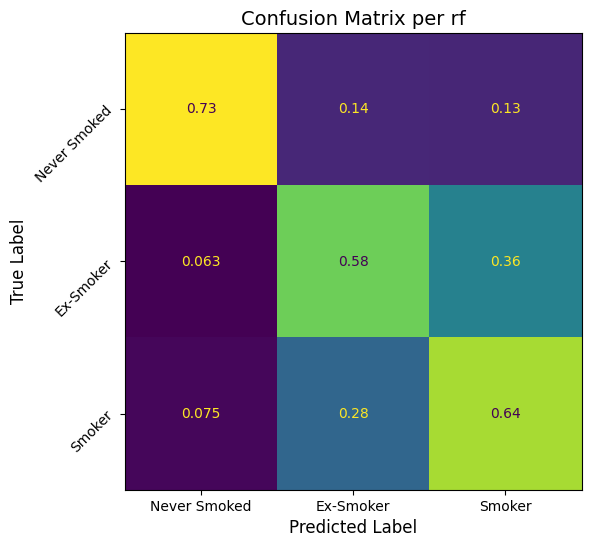
\includegraphics[width=\columnwidth,height=0.75\columnwidth,keepaspectratio]{screen_results/confusion_matrix_feature_engeneering_rf_s.png}
\end{minipage}
\end{center}

\subsection*{AdaBoost (Smoke)}
\begin{center}
\begin{minipage}[c]{0.50\columnwidth}
\resizebox{\columnwidth}{!}{%
\begin{tabular}{lcccc}
\toprule
Label        & Precision & Recall & F1-score & Support \\
\midrule
Non-smoker   & 0.83      & 0.83   & 0.83     & 120489 \\
Ex-smoker    & 0.44      & 0.32   & 0.37     & 34990  \\
Smoker       & 0.51      & 0.62   & 0.56     & 42791  \\
\midrule
Accuracy     & --        & --     & 0.70     & 198270 \\
Macro avg    & 0.59      & 0.59   & 0.59     & 198270 \\
Weighted avg & 0.69      & 0.70   & 0.69     & 198270 \\
\bottomrule
\end{tabular}%
}
\end{minipage}\hspace{\columnsep}%
\begin{minipage}[c]{0.40\columnwidth}
\centering
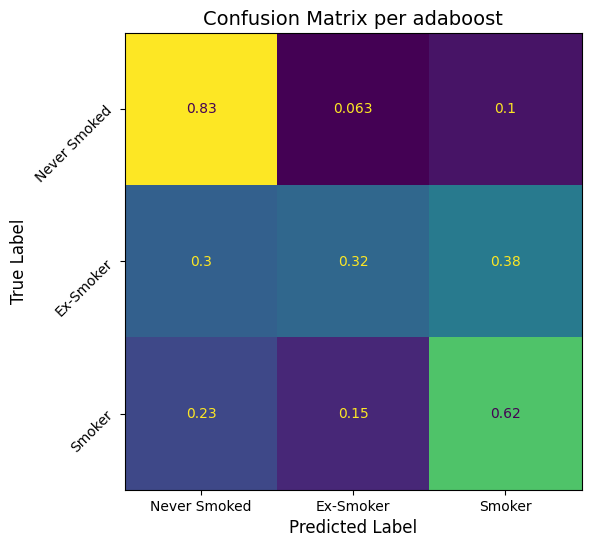
\includegraphics[width=\columnwidth,height=0.75\columnwidth,keepaspectratio]{screen_results/confusion_matrix_feature_engeneering_adaboost_s.png}
\end{minipage}
\end{center}

\subsection*{SVM (Smoke)}
\begin{center}
\begin{minipage}[c]{0.50\columnwidth}
\resizebox{\columnwidth}{!}{%
\begin{tabular}{lcccc}
\toprule
Label        & Precision & Recall & F1-score & Support \\
\midrule
Non-smoker   & 0.94      & 0.73   & 0.82     & 120489 \\
Ex-smoker    & 0.41      & 0.55   & 0.47     & 34990  \\
Smoker       & 0.48      & 0.65   & 0.55     & 42791  \\
\midrule
Accuracy     & --        & --     & 0.68     & 198270 \\
Macro avg    & 0.61      & 0.64   & 0.61     & 198270 \\
Weighted avg & 0.75      & 0.68   & 0.70     & 198270 \\
\bottomrule
\end{tabular}%
}
\end{minipage}\hspace{\columnsep}%
\begin{minipage}[c]{0.40\columnwidth}
\centering
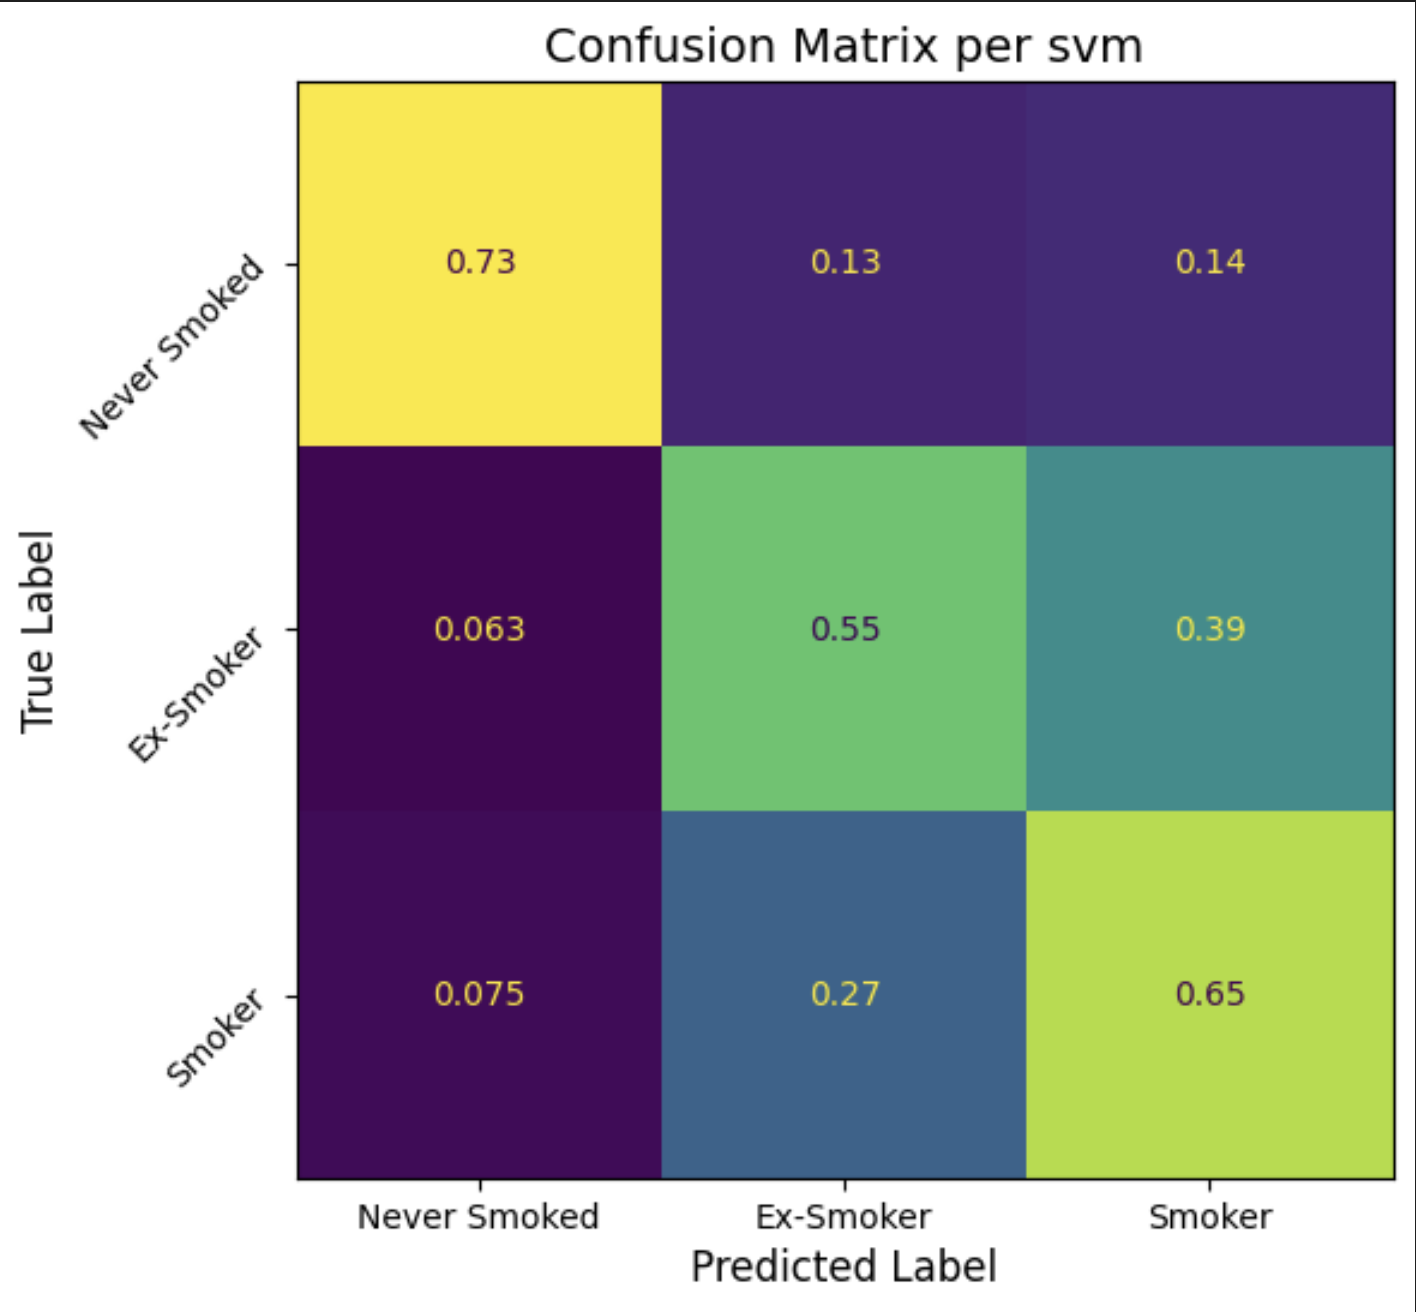
\includegraphics[width=\columnwidth,height=0.75\columnwidth,keepaspectratio]{screen_results/confusion_matrix_feature_engeneering_svm_s.png}
\end{minipage}
\end{center}

\subsection*{KNN (Smoke)}
\begin{center}
\begin{minipage}[c]{0.50\columnwidth}
\resizebox{\columnwidth}{!}{%
\begin{tabular}{lcccc}
\toprule
Label        & Precision & Recall & F1-score & Support \\
\midrule
Non-smoker   & 0.84      & 0.81   & 0.83     & 120489 \\
Ex-smoker    & 0.43      & 0.38   & 0.41     & 34990  \\
Smoker       & 0.49      & 0.58   & 0.53     & 42791  \\
\midrule
Accuracy     & --        & --     & 0.69     & 198270 \\
Macro avg    & 0.59      & 0.59   & 0.59     & 198270 \\
Weighted avg & 0.69      & 0.69   & 0.69     & 198270 \\
\bottomrule
\end{tabular}%
}
\end{minipage}\hspace{\columnsep}%
\begin{minipage}[c]{0.40\columnwidth}
\centering
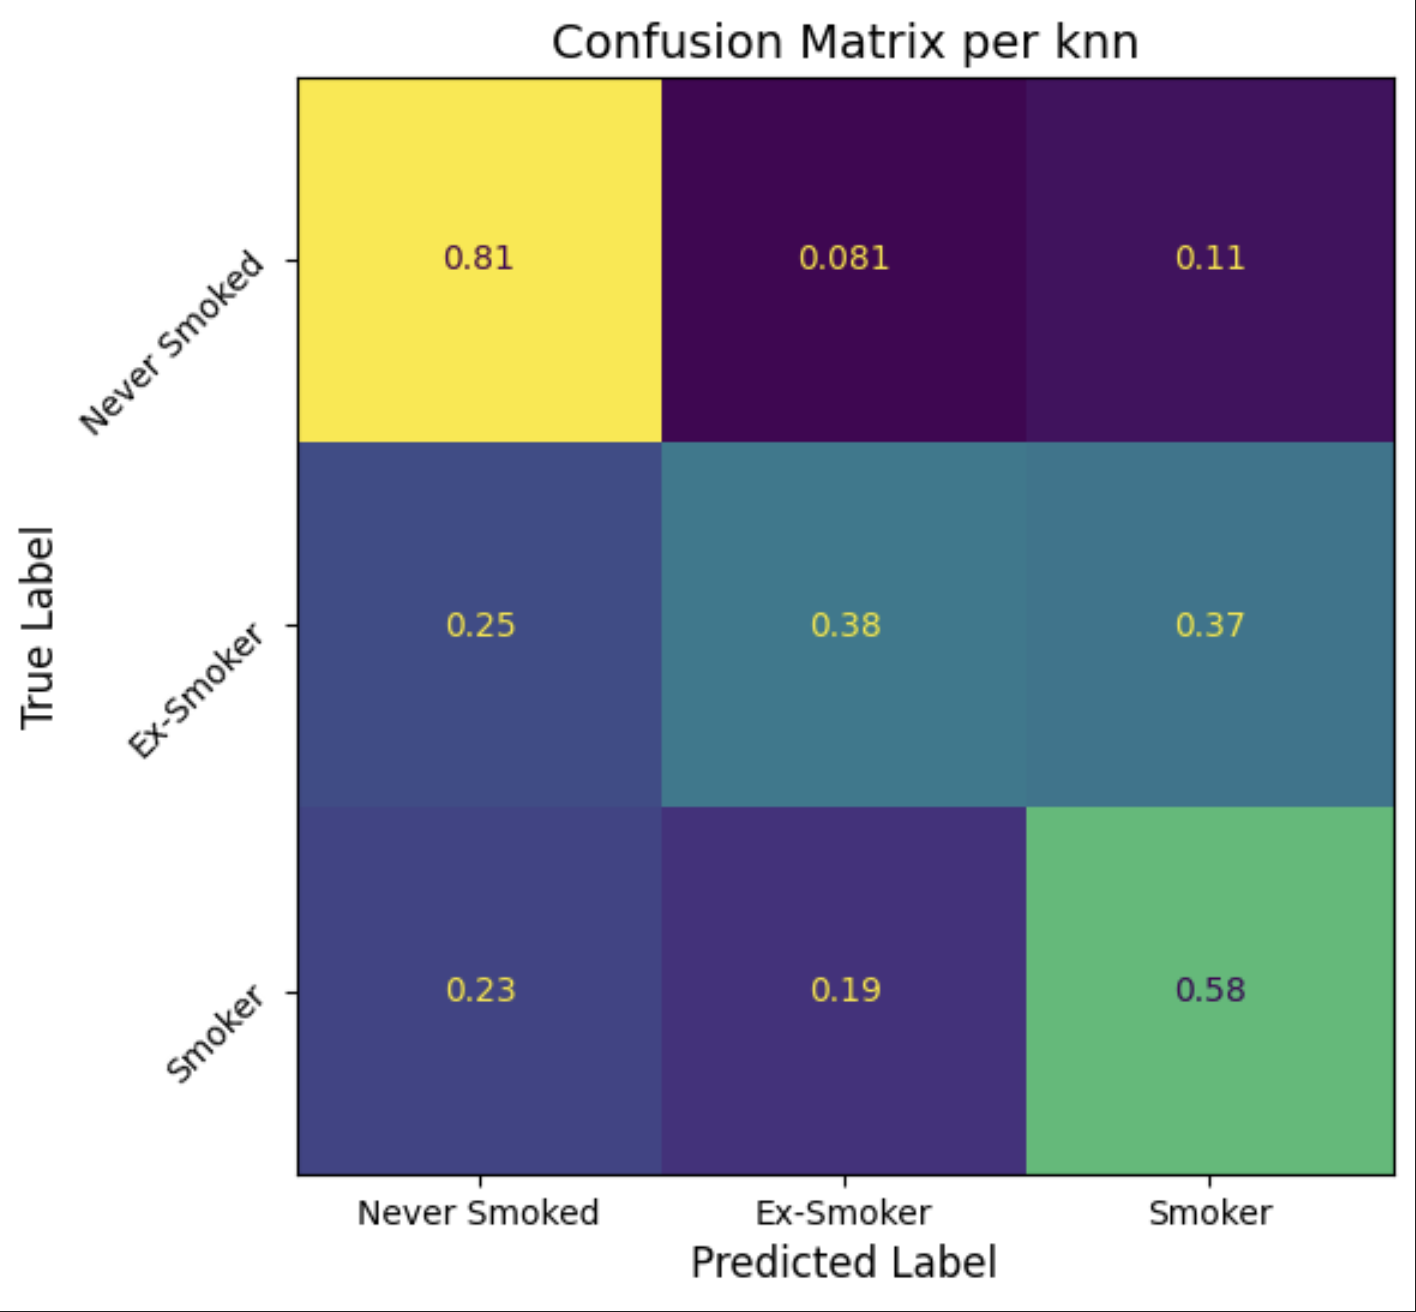
\includegraphics[width=\columnwidth,height=0.75\columnwidth,keepaspectratio]{screen_results/confusion_matrix_feature_engeneering_knn_s.png}
\end{minipage}
\end{center}

\subsection*{Random Forest (Drink)}
\begin{center}
\begin{minipage}[c]{0.50\columnwidth}
\resizebox{\columnwidth}{!}{%
\begin{tabular}{lcccc}
\toprule
Label & Precision & Recall & F1-score & Support \\
\midrule
Y     & 0.74      & 0.72   & 0.73     & 99172 \\
N     & 0.73      & 0.75   & 0.74     & 99098 \\
\midrule
Accuracy     & --        & --     & 0.73     & 198270 \\
Macro avg    & 0.73      & 0.73   & 0.73     & 198270 \\
Weighted avg & 0.73      & 0.73   & 0.73     & 198270 \\
\bottomrule
\end{tabular}%
}
\end{minipage}\hspace{\columnsep}%
\begin{minipage}[c]{0.40\columnwidth}
\centering
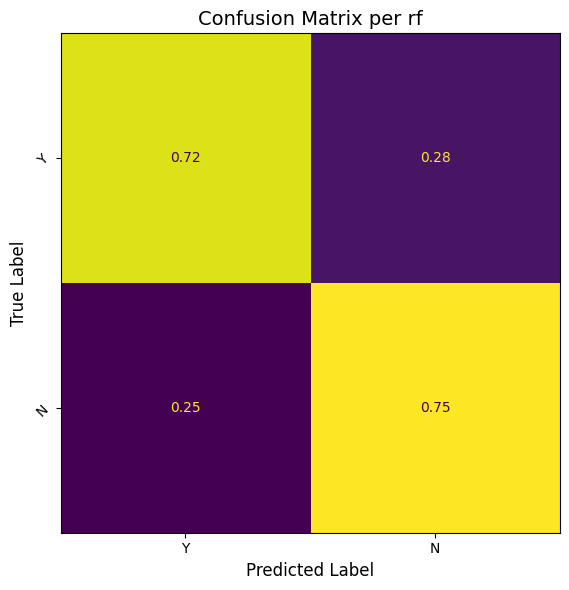
\includegraphics[width=\columnwidth,height=0.75\columnwidth,keepaspectratio]{screen_results/confusion_matrix_feature_engeneering_rf_d.png}
\end{minipage}
\end{center}

\subsection*{AdaBoost (Drink)}
\begin{center}
\begin{minipage}[c]{0.50\columnwidth}
\resizebox{\columnwidth}{!}{%
\begin{tabular}{lcccc}
\toprule
Label & Precision & Recall & F1-score & Support \\
\midrule
Y     & 0.73      & 0.73   & 0.73     & 99172 \\
N     & 0.73      & 0.73   & 0.73     & 99098 \\
\midrule
Accuracy     & --        & --     & 0.73     & 198270 \\
Macro avg    & 0.73      & 0.73   & 0.73     & 198270 \\
Weighted avg & 0.73      & 0.73   & 0.73     & 198270 \\
\bottomrule
\end{tabular}%
}
\end{minipage}\hspace{\columnsep}%
\begin{minipage}[c]{0.40\columnwidth}
\centering
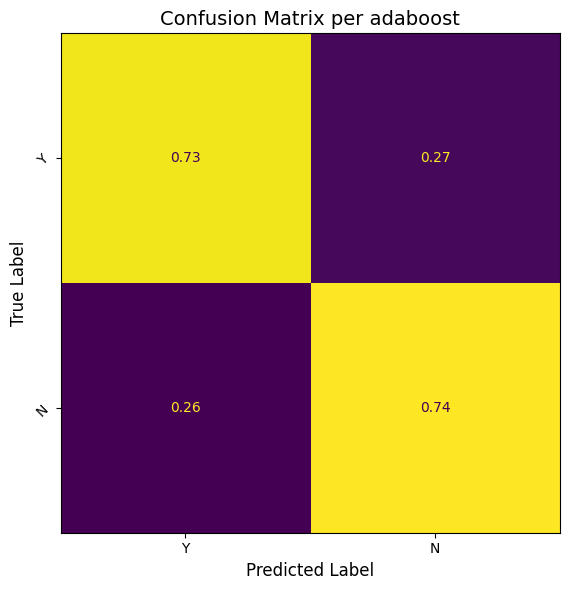
\includegraphics[width=\columnwidth,height=0.75\columnwidth,keepaspectratio]{screen_results/confusion_matrix_feature_engeneering_adaboost_d.png}
\end{minipage}
\end{center}

\subsection*{SVM (Drink)}
\begin{center}
\begin{minipage}[c]{0.50\columnwidth}
\resizebox{\columnwidth}{!}{%
\begin{tabular}{lcccc}
\toprule
Label & Precision & Recall & F1-score & Support \\
\midrule
Y     & 0.73      & 0.72   & 0.72     & 99172 \\
N     & 0.72      & 0.73   & 0.72     & 99098 \\
\midrule
Accuracy     & --        & --     & 0.72     & 198270 \\
Macro avg    & 0.72      & 0.72   & 0.72     & 198270 \\
Weighted avg & 0.72      & 0.72   & 0.72     & 198270 \\
\bottomrule
\end{tabular}%
}
\end{minipage}\hspace{\columnsep}%
\begin{minipage}[c]{0.40\columnwidth}
\centering
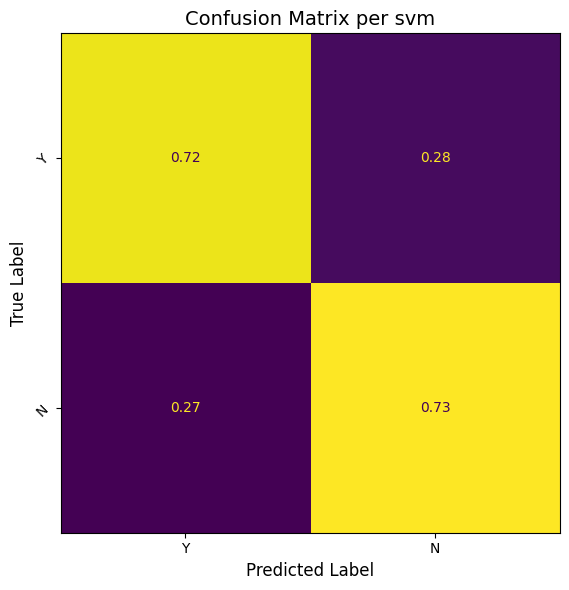
\includegraphics[width=\columnwidth,height=0.75\columnwidth,keepaspectratio]{screen_results/confusion_matrix_feature_engeneering_svm_d.png}
\end{minipage}
\end{center}

\subsection*{KNN (Drink)}
\begin{center}
\begin{minipage}[c]{0.50\columnwidth}
\resizebox{\columnwidth}{!}{%
\begin{tabular}{lcccc}
\toprule
Label & Precision & Recall & F1-score & Support \\
\midrule
Y     & 0.73      & 0.67   & 0.70     & 99172 \\
N     & 0.70      & 0.76   & 0.73     & 99098 \\
\midrule
Accuracy     & --        & --     & 0.71     & 198270 \\
Macro avg    & 0.72      & 0.71   & 0.71     & 198270 \\
Weighted avg & 0.72      & 0.71   & 0.71     & 198270 \\
\bottomrule
\end{tabular}%
}
\end{minipage}\hspace{\columnsep}%
\begin{minipage}[c]{0.40\columnwidth}
\centering
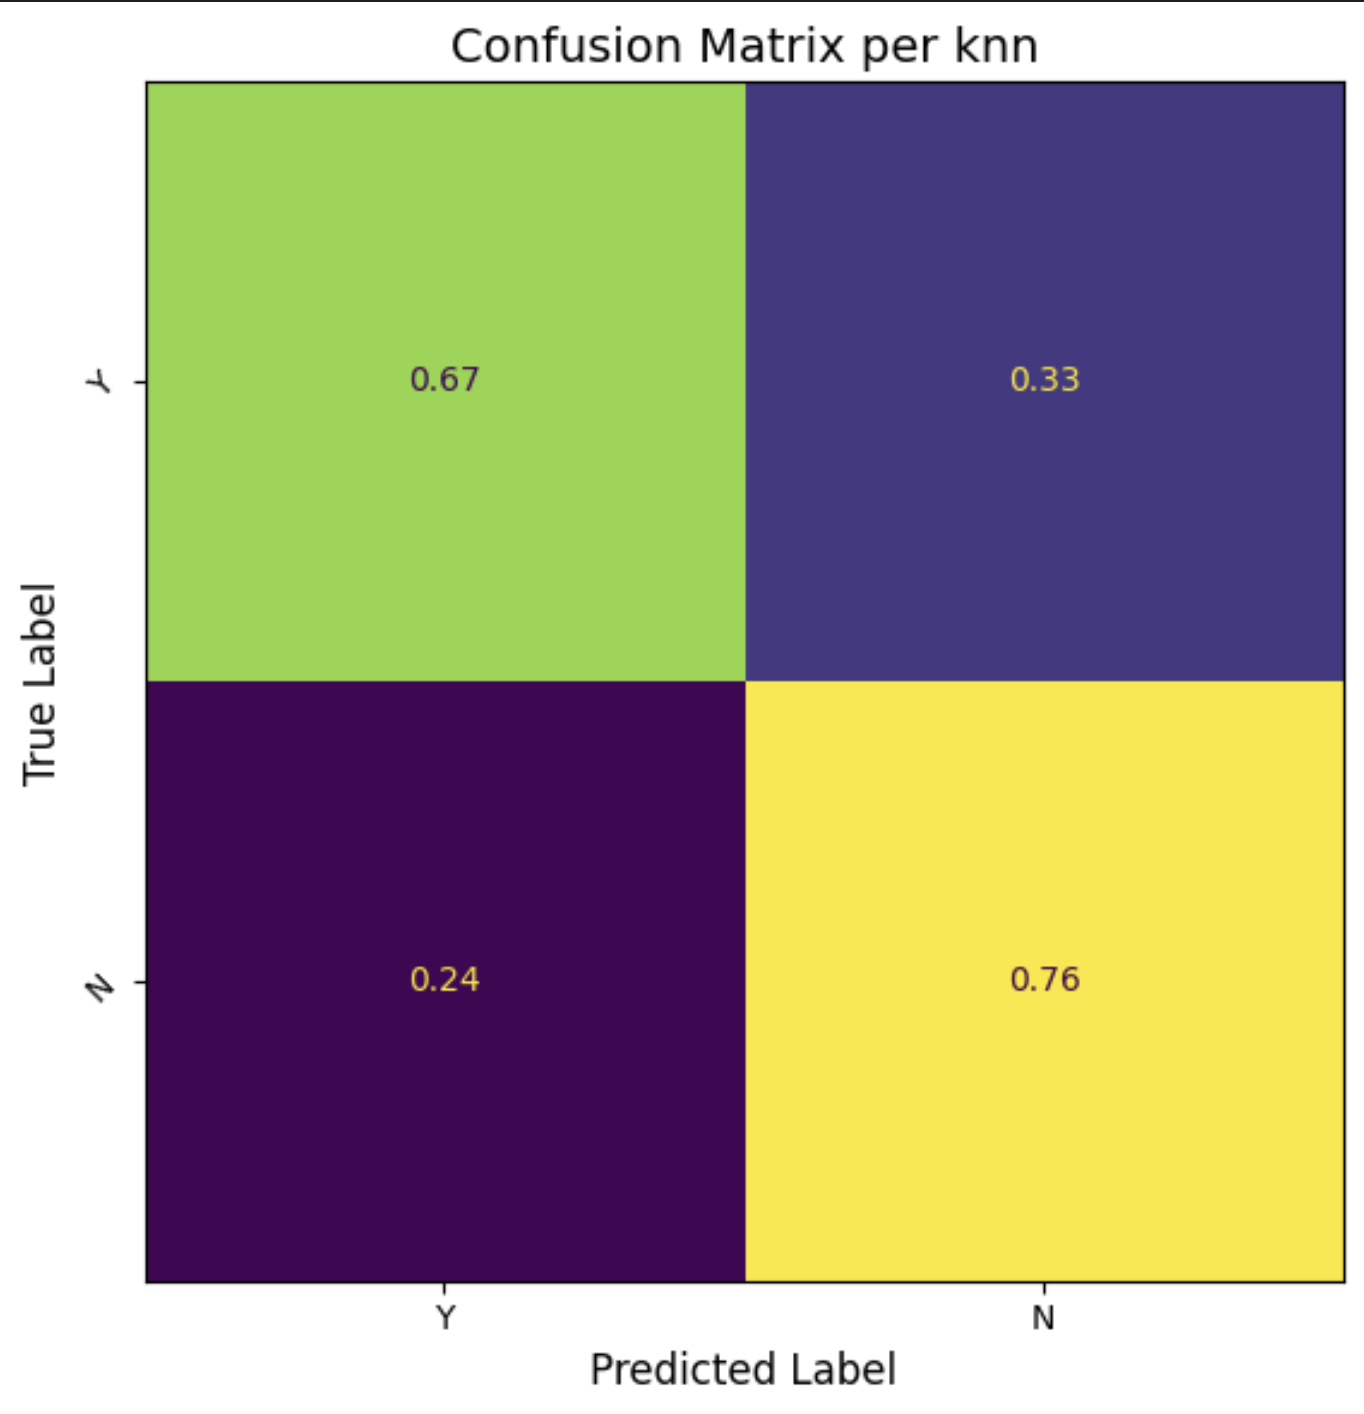
\includegraphics[width=\columnwidth,height=0.75\columnwidth,keepaspectratio]{screen_results/confusion_matrix_feature_engeneering_knn_d.png}
\end{minipage}
\end{center}

%%%%%%%%%%%%%%%%%%%%%%%%%%%%%%%%%%%%%%%%%%%%%%%%%%%%%%%%%%%%%%%%%%%%%%%%%%%%%%
% Feature Engeneering con PCA (SVM, KNN)
%%%%%%%%%%%%%%%%%%%%%%%%%%%%%%%%%%%%%%%%%%%%%%%%%%%%%%%%%%%%%%%%%%%%%%%%%%%%%%

\subsection{Feature Engeneering con PCA (SVM, KNN)}
Per la stessa ragione del caso senza feature engeneering, abbiamo ritenuto opportuno provare ad applicare una PCA ai modelli SVM e KNN; per di più aver aumentato il numero di feature, ha imcrementato la dimensionalità del dataset e dunque abbiamo ritenuto opportuno apllicare una tecnica di dimensionality reduction per cercare di estrarre eventualmente dei pattern più significativi.

\subsection*{SVM (Smoke) }
\begin{center}
\begin{minipage}[c]{0.50\columnwidth}
\resizebox{\columnwidth}{!}{%
\begin{tabular}{lcccc}
\toprule
Label        & Precision & Recall & F1-score & Support \\
\midrule
Non-smoker   & 0.89      & 0.76   & 0.82     & 120489 \\
Ex-smoker    & 0.41      & 0.44   & 0.43     & 34990  \\
Smoker       & 0.48      & 0.63   & 0.54     & 42791  \\
\midrule
Accuracy     & --        & --     & 0.68     & 198270 \\
Macro avg    & 0.59      & 0.61   & 0.60     & 198270 \\
Weighted avg & 0.71      & 0.68   & 0.69     & 198270 \\
\bottomrule
\end{tabular}%
}
\end{minipage}\hspace{\columnsep}%
\begin{minipage}[c]{0.40\columnwidth}
\centering
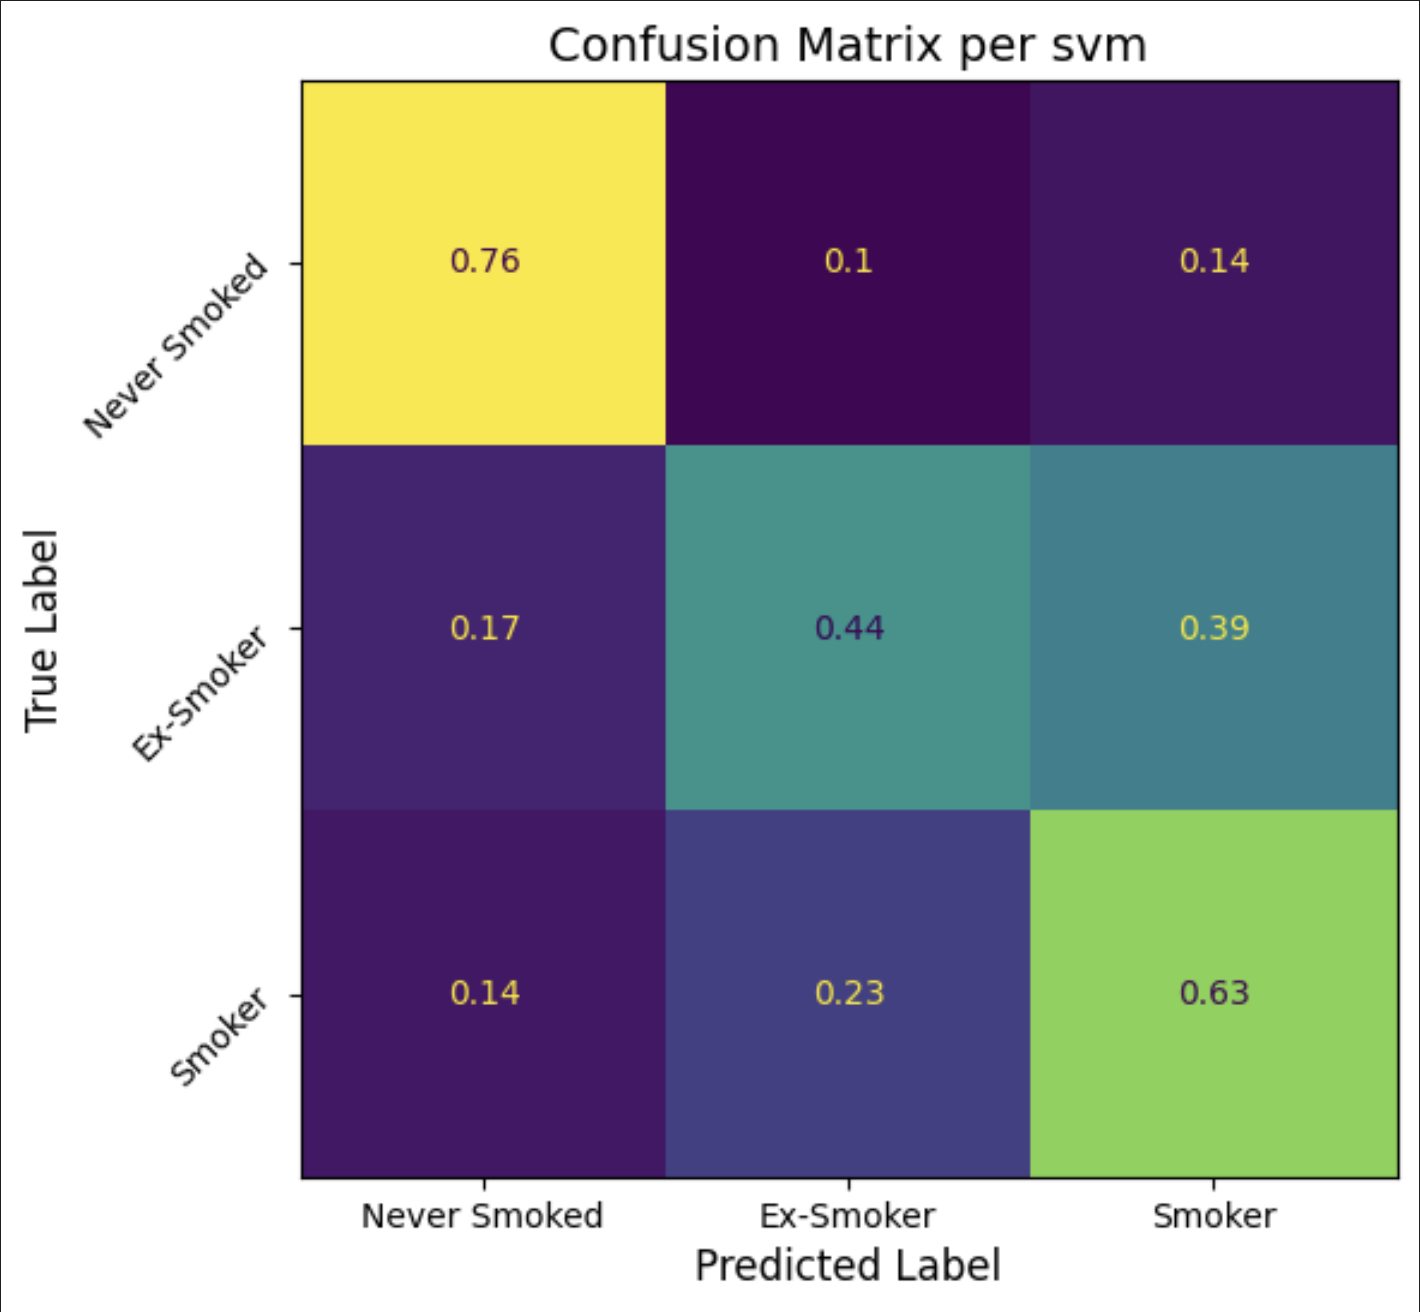
\includegraphics[width=\columnwidth,height=0.75\columnwidth,keepaspectratio]{screen_results/confusion_matrix_feature_engeneering_pca_svm_s.png}
\end{minipage}
\end{center}

\subsection*{KNN (Smoke) }
\begin{center}
\begin{minipage}[c]{0.50\columnwidth}
\resizebox{\columnwidth}{!}{%
\begin{tabular}{lcccc}
\toprule
Label        & Precision & Recall & F1-score & Support \\
\midrule
Non-smoker   & 0.82      & 0.82   & 0.82     & 120489 \\
Ex-smoker    & 0.43      & 0.34   & 0.38     & 34990  \\
Smoker       & 0.49      & 0.57   & 0.53     & 42791  \\
\midrule
Accuracy     & --        & --     & 0.68     & 198270 \\
Macro avg    & 0.58      & 0.58   & 0.58     & 198270 \\
Weighted avg & 0.68      & 0.68   & 0.68     & 198270 \\
\bottomrule
\end{tabular}%
}
\end{minipage}\hspace{\columnsep}%
\begin{minipage}[c]{0.40\columnwidth}
\centering
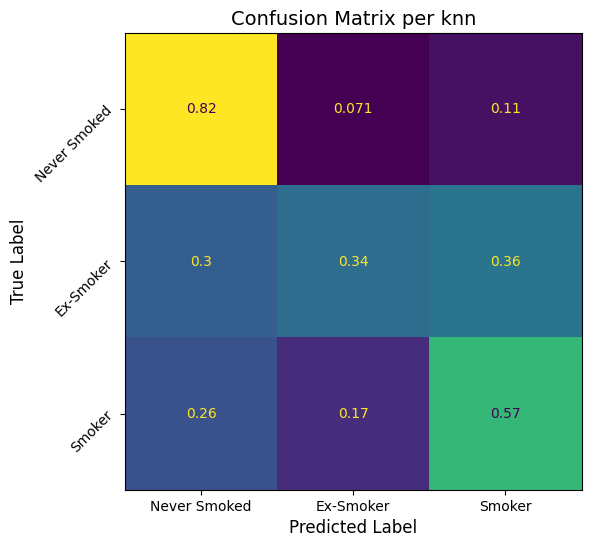
\includegraphics[width=\columnwidth,height=0.75\columnwidth,keepaspectratio]{screen_results/confusion_matrix_feature_engeneering_pca_knn_s.png}
\end{minipage}
\end{center}

\subsection*{SVM (Drink) }
\begin{center}
\begin{minipage}[c]{0.50\columnwidth}
\resizebox{\columnwidth}{!}{%
\begin{tabular}{lcccc}
\toprule
Label & Precision & Recall & F1-score & Support \\
\midrule
Y     & 0.72      & 0.72   & 0.72     & 99172 \\
N     & 0.72      & 0.72   & 0.72     & 99098 \\
\midrule
Accuracy     & --        & --     & 0.72     & 198270 \\
Macro avg    & 0.72      & 0.72   & 0.72     & 198270 \\
Weighted avg & 0.72      & 0.72   & 0.72     & 198270 \\
\bottomrule
\end{tabular}%
}
\end{minipage}\hspace{\columnsep}%
\begin{minipage}[c]{0.40\columnwidth}
\centering
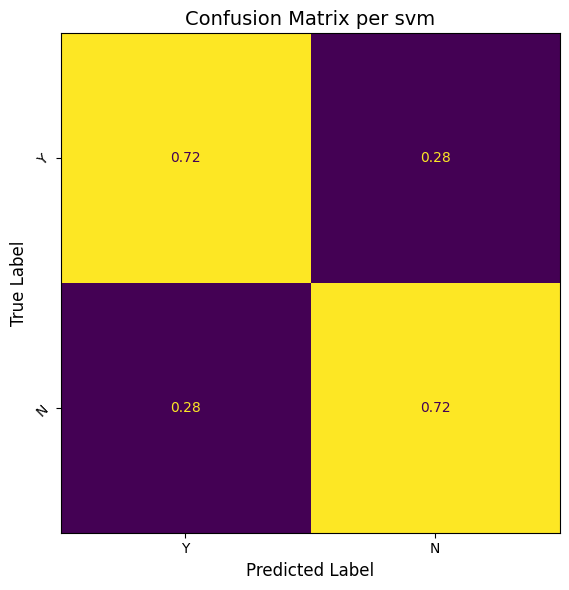
\includegraphics[width=\columnwidth,height=0.75\columnwidth,keepaspectratio]{screen_results/confusion_matrix_feature_engeneering_pca_svm_d.png}
\end{minipage}
\end{center}

\subsection*{KNN (Drink) }
\begin{center}
\begin{minipage}[c]{0.50\columnwidth}
\resizebox{\columnwidth}{!}{%
\begin{tabular}{lcccc}
\toprule
Label & Precision & Recall & F1-score & Support \\
\midrule
Y     & 0.73      & 0.68   & 0.70     & 99172 \\
N     & 0.70      & 0.75   & 0.72     & 99098 \\
\midrule
Accuracy     & --        & --     & 0.71     & 198270 \\
Macro avg    & 0.71      & 0.71   & 0.71     & 198270 \\
Weighted avg & 0.71      & 0.71   & 0.71     & 198270 \\
\bottomrule
\end{tabular}%
}
\end{minipage}\hspace{\columnsep}%
\begin{minipage}[c]{0.40\columnwidth}
\centering
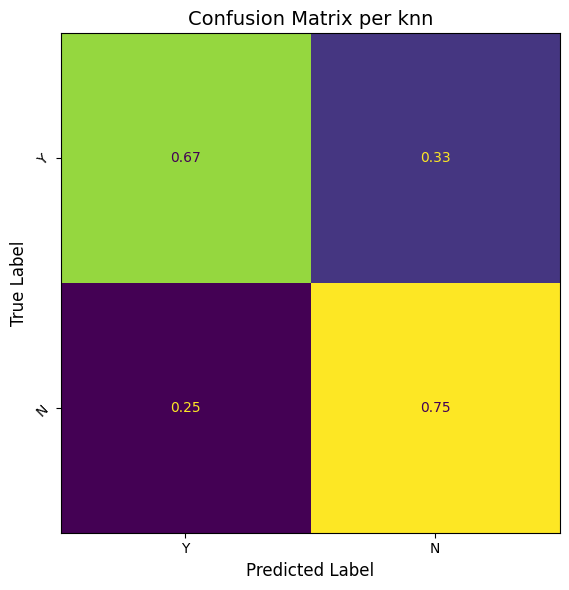
\includegraphics[width=\columnwidth,height=0.75\columnwidth,keepaspectratio]{screen_results/confusion_matrix_knn_pca_d.png}
\end{minipage}
\end{center}

%%%%%%%%%%%%%%%%%%%%%%%%%%%%%%%%%%%%%%%%%%%%%%%%%%%%%%%%%%%%%%%%%%%%%%%%%%%%%%
% Bagging Ensemble
%%%%%%%%%%%%%%%%%%%%%%%%%%%%%%%%%%%%%%%%%%%%%%%%%%%%%%%%%%%%%%%%%%%%%%%%%%%%%%

\subsection{Bagging Ensemble}
Siccome il tempo di train di un modello di tipo SVM con kernel non lineare cresce quadraticamente con la grandezza del dataset, si è reso impossibile testare un modello di questo tipo; come soluzione per provare comunque a osservare se fosse possibile ottenere dei risultati interessanti con tale modello, abbiamo provato utilizzare la tecnica di predizione del Bagging Ensemble.
C'è da specificare che ogni modello base di SVM non lineare è stato allenato solo sul 10\% del dataset, dunque i risultati non sono apprezzabili totalmente.
Inoltre, per testare anche la combinazione della tecnica del Bagging con quella del Boosting, in questo tipo di test abbiamo utilizzato anche il classificatore AdaBoost.

\subsection*{AdaBoost (Smoke)}
\begin{center}
\begin{minipage}[c]{0.50\columnwidth}
\resizebox{\columnwidth}{!}{%
\begin{tabular}{lcccc}
\toprule
Label        & Precision & Recall & F1-score & Support \\
\midrule
Non-smoker   & 0.84      & 0.82   & 0.83     & 120582 \\
Ex-smoker    & 0.44      & 0.27   & 0.34     & 34919  \\
Smoker       & 0.49      & 0.65   & 0.56     & 42769  \\
\midrule
Accuracy     & --        & --     & 0.69     & 198270 \\
Macro avg    & 0.59      & 0.58   & 0.57     & 198270 \\
Weighted avg & 0.69      & 0.69   & 0.68     & 198270 \\
\bottomrule
\end{tabular}%
}
\end{minipage}\hspace{\columnsep}%
\begin{minipage}[c]{0.40\columnwidth}
\centering
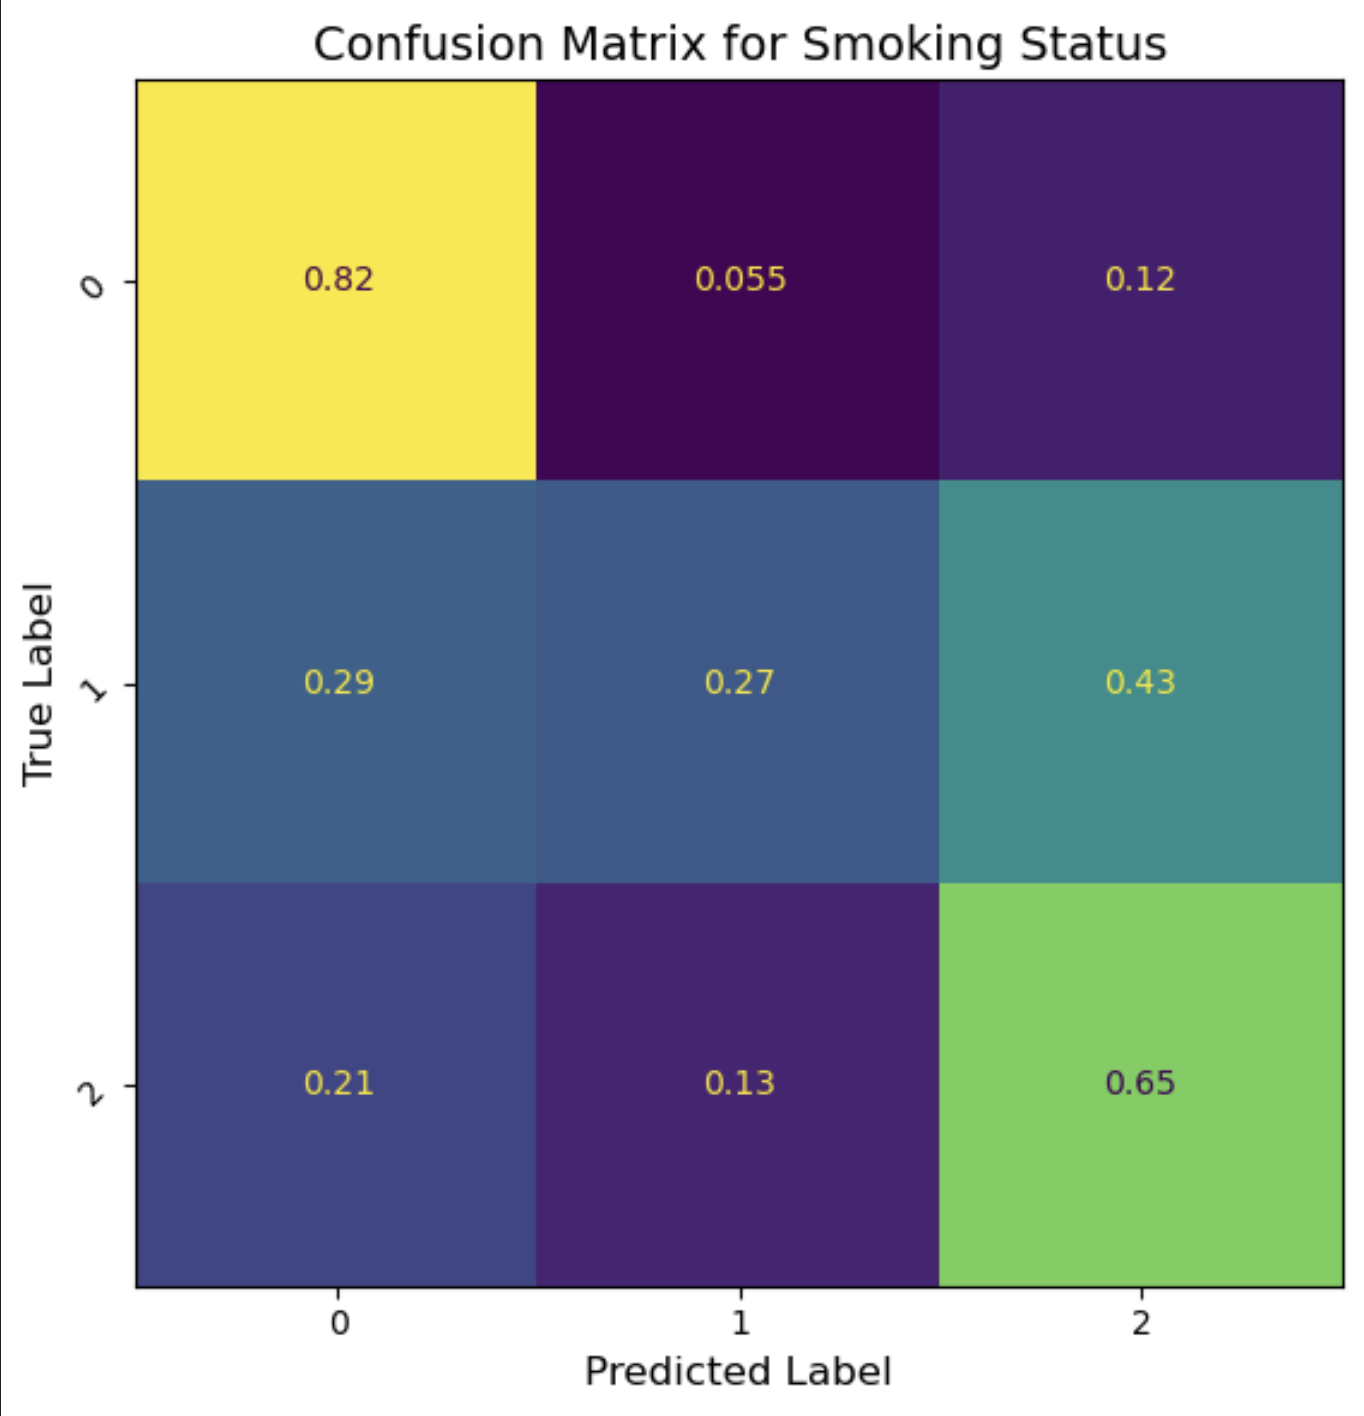
\includegraphics[width=\columnwidth,height=0.75\columnwidth,keepaspectratio]{screen_results/confusion_matrix_bagging_adaboost_s.png}
\end{minipage}
\end{center}

\subsection*{AVM (Smoke)}
\begin{center}
\begin{minipage}[c]{0.50\columnwidth}
\resizebox{\columnwidth}{!}{%
\begin{tabular}{lcccc}
\toprule
Label        & Precision & Recall & F1-score & Support \\
\midrule
Non-smoker   & 0.82      & 0.84   & 0.83     & 120582 \\
Ex-smoker    & 0.45      & 0.31   & 0.37     & 34919  \\
Smoker       & 0.50      & 0.59   & 0.54     & 42769  \\
\midrule
Accuracy     & --        & --     & 0.69     & 198270 \\
Macro avg    & 0.59      & 0.58   & 0.58     & 198270 \\
Weighted avg & 0.68      & 0.69   & 0.68     & 198270 \\
\bottomrule
\end{tabular}%
}
\end{minipage}\hspace{\columnsep}%
\begin{minipage}[c]{0.40\columnwidth}
\centering
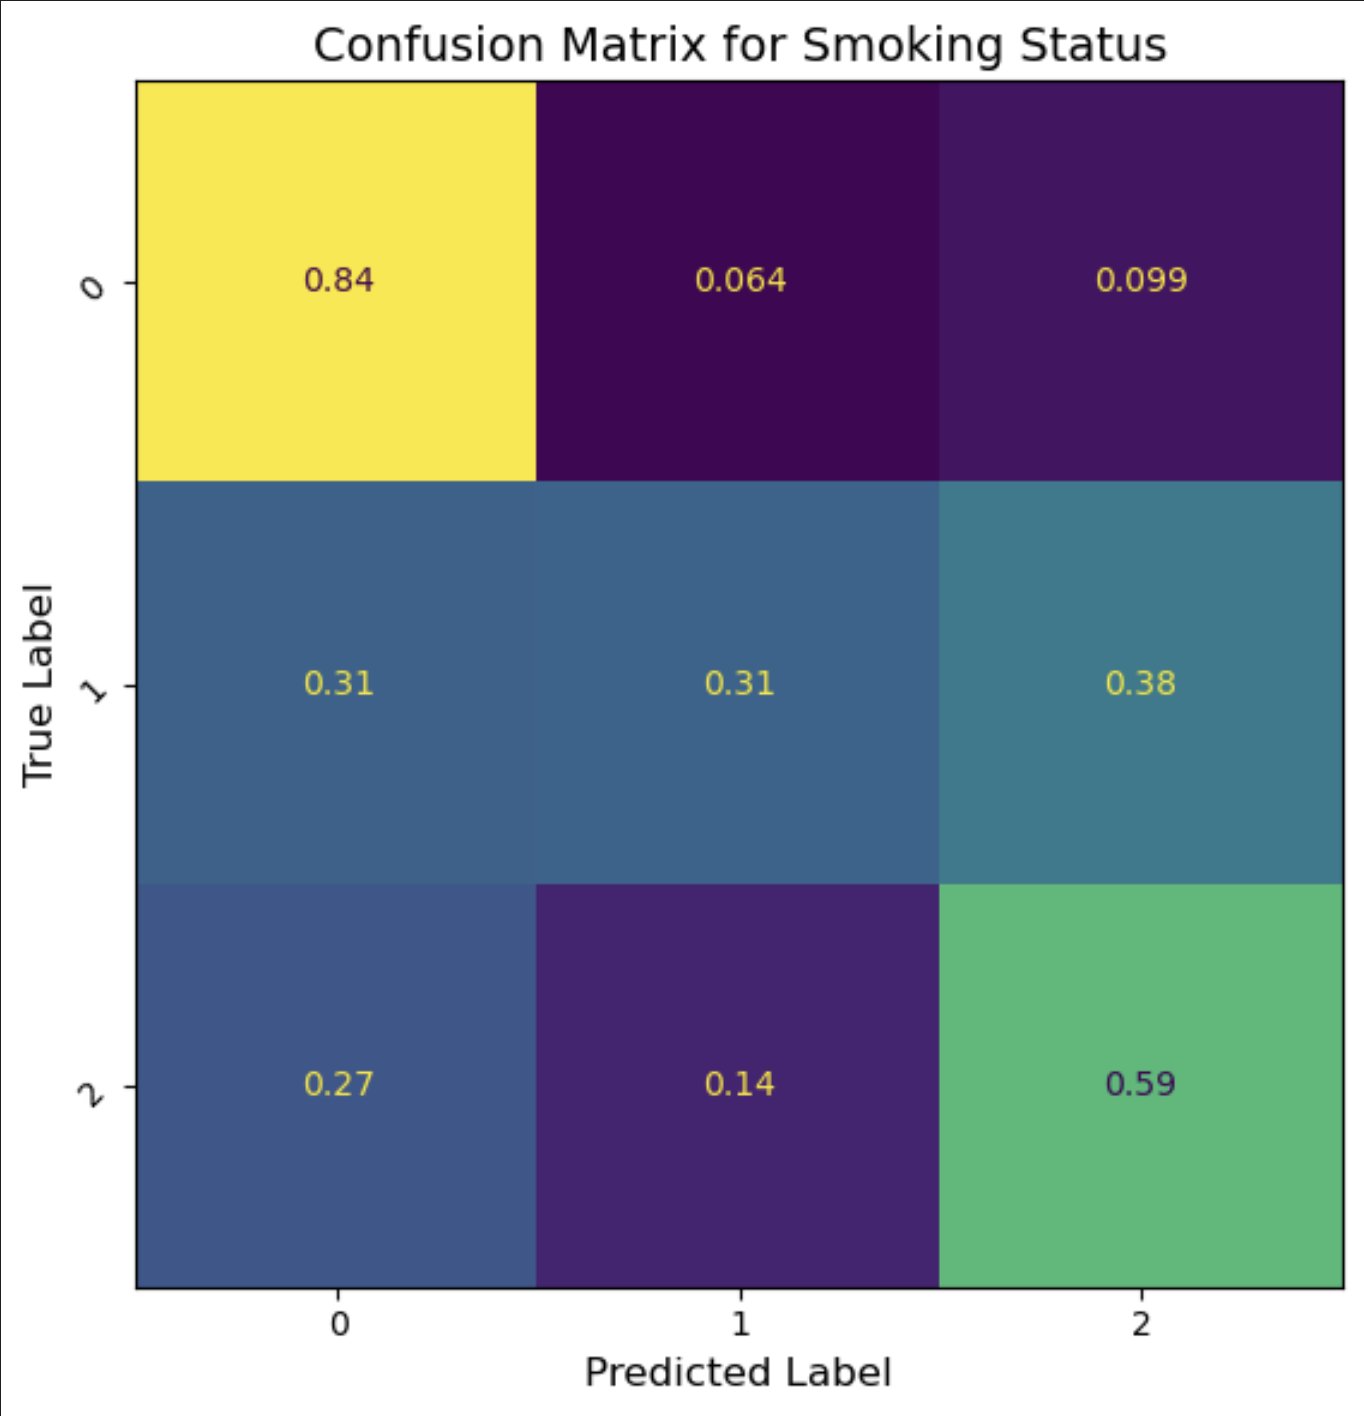
\includegraphics[width=\columnwidth,height=0.75\columnwidth,keepaspectratio]{screen_results/confusion_matrix_bagging_svm_s.png}
\end{minipage}
\end{center}

\subsection*{AdaBoost (Drink)}
\begin{center}
\begin{minipage}[c]{0.50\columnwidth}
\resizebox{\columnwidth}{!}{%
\begin{tabular}{lcccc}
\toprule
Label & Precision & Recall & F1-score & Support \\
\midrule
Y     & 0.72      & 0.73   & 0.72     & 99595 \\
N     & 0.72      & 0.72   & 0.72     & 98675 \\
\midrule
Accuracy     & --        & --     & 0.72     & 198270 \\
Macro avg    & 0.72      & 0.72   & 0.72     & 198270 \\
Weighted avg & 0.72      & 0.72   & 0.72     & 198270 \\
\bottomrule
\end{tabular}%
}
\end{minipage}\hspace{\columnsep}%
\begin{minipage}[c]{0.40\columnwidth}
\centering
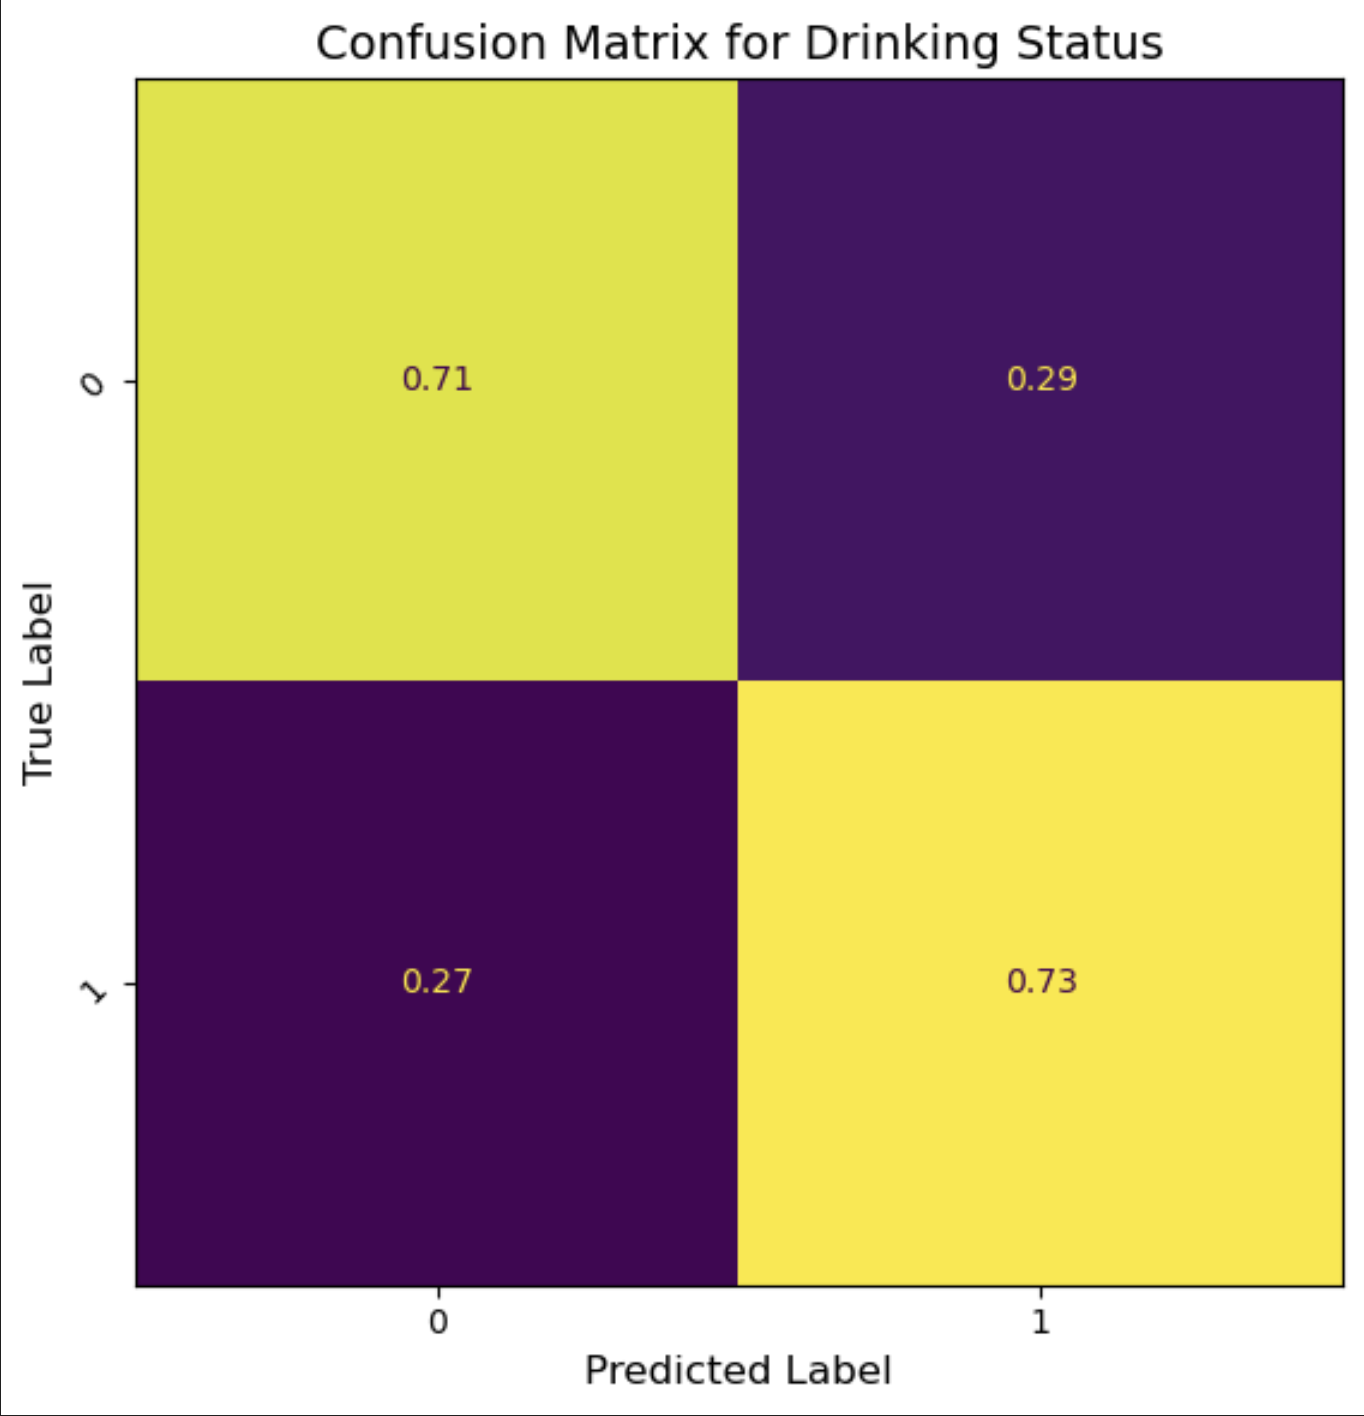
\includegraphics[width=\columnwidth,height=0.75\columnwidth,keepaspectratio]{screen_results/confusion_matrix_bagging_svm_d.png}
\end{minipage}
\end{center}

\subsection*{SVM (Drink)}
\begin{center}
\begin{minipage}[c]{0.50\columnwidth}
\resizebox{\columnwidth}{!}{%
\begin{tabular}{lcccc}
\toprule
Label & Precision & Recall & F1-score & Support \\
\midrule
Y     & 0.73      & 0.71   & 0.72     & 99595 \\
N     & 0.72      & 0.73   & 0.73     & 98675 \\
\midrule
Accuracy     & --        & --     & 0.72     & 198270 \\
Macro avg    & 0.72      & 0.72   & 0.72     & 198270 \\
Weighted avg & 0.72      & 0.72   & 0.72     & 198270 \\
\bottomrule
\end{tabular}%
}
\end{minipage}\hspace{\columnsep}%
\begin{minipage}[c]{0.40\columnwidth}
\centering
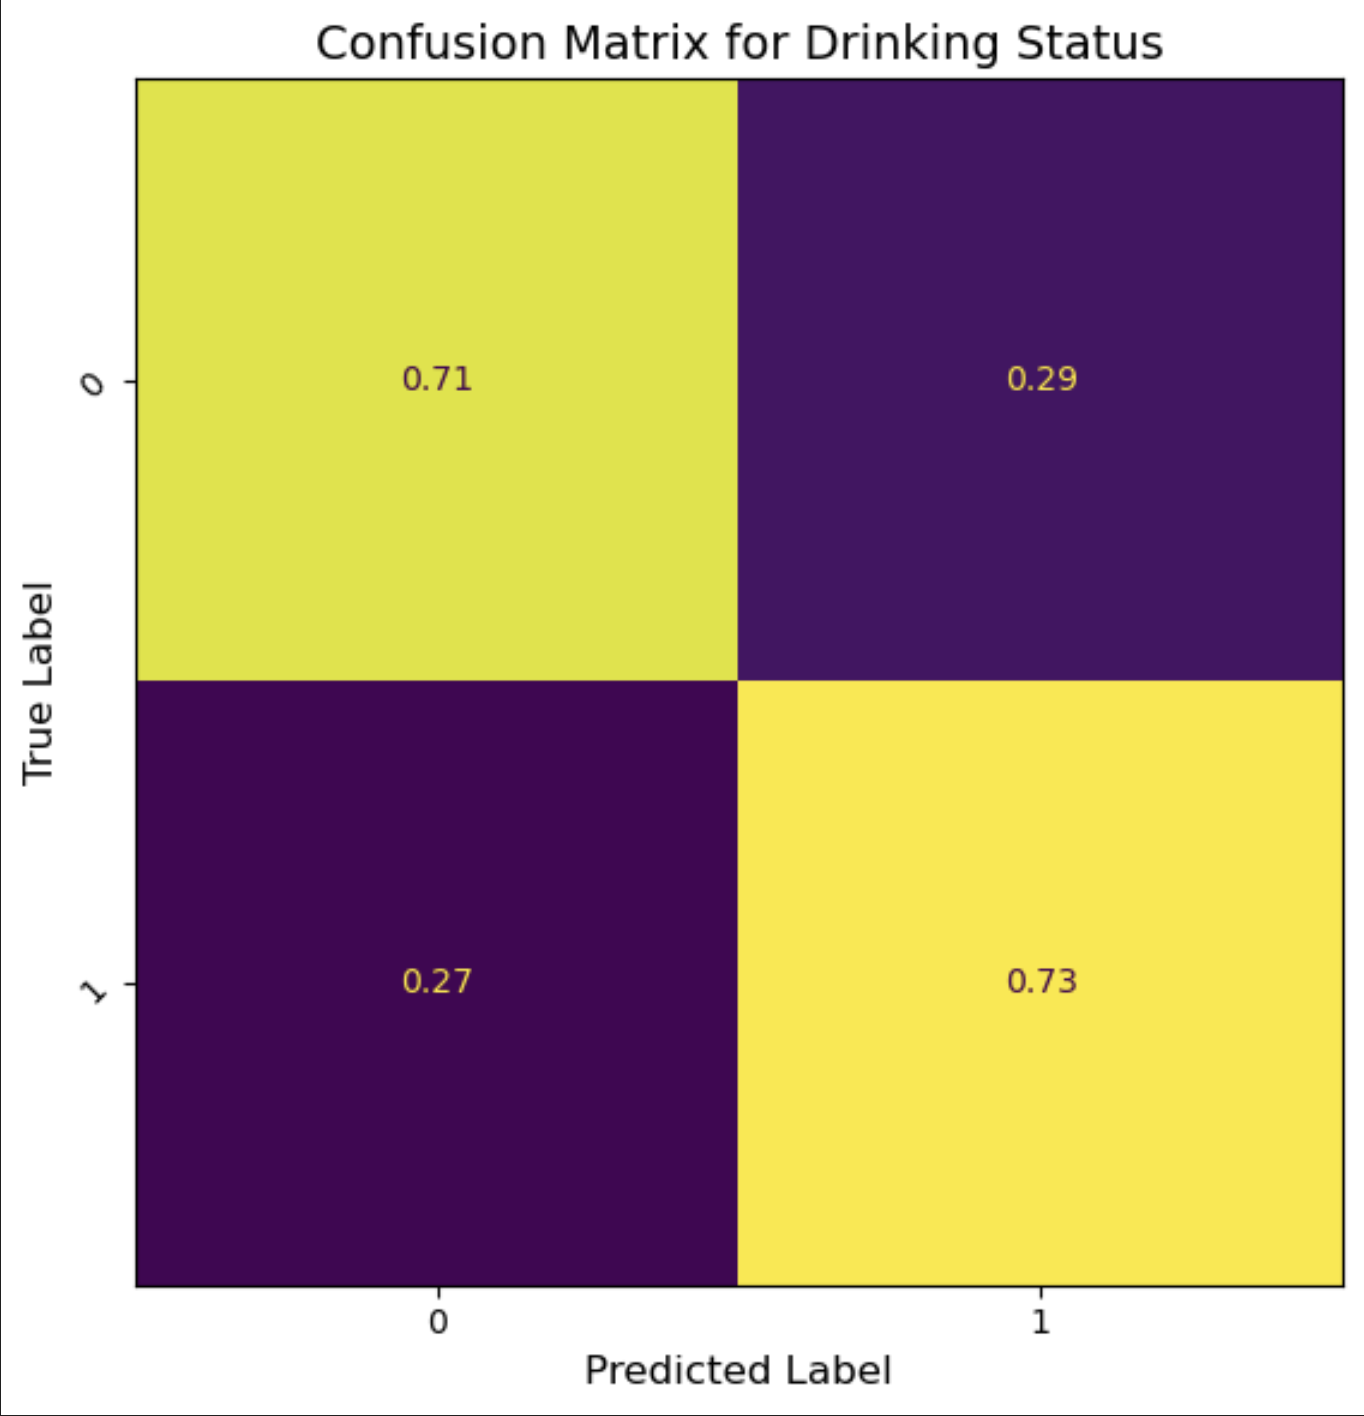
\includegraphics[width=\columnwidth,height=0.75\columnwidth,keepaspectratio]{screen_results/confusion_matrix_bagging_svm_d.png}
\end{minipage}
\end{center}

%%%%%%%%%%%%%%%%%%%%%%%%%%%%%%%%%%%%%%%%%%%%%%%%%%%%%%%%%%%%%%%%%%%%%%%%%%%%%%
% Stacking Classifier e Voting Classifier
%%%%%%%%%%%%%%%%%%%%%%%%%%%%%%%%%%%%%%%%%%%%%%%%%%%%%%%%%%%%%%%%%%%%%%%%%%%%%%

\subsection{Stacking Classifier e Voting Classifier}
Uno dei nostri ultimi tentativi di migliorare i risultati della Random Forest, è stato quello di sfruttare due tecniche di Ensemble differenti dal Bagging ed il Boosting: lo Stacking ed il Voting Classifier; abbiamo pensato infatti che potesse essere conveniente combinare la predizione proveniente da modelli diversi come filosofia, però purtroppo anche per quanto riguarda questo test abbiamo ottenuto più o meno gli stessi risultati.

\subsection*{Stacking (Smoke)}
\begin{center}
\begin{minipage}[c]{0.50\columnwidth}
\resizebox{\columnwidth}{!}{%
\begin{tabular}{lcccc}
\toprule
Label        & Precision & Recall & F1-score & Support \\
\midrule
Non-smoker   & 0.89      & 0.79   & 0.83     & 111686 \\
Ex-smoker    & 0.44      & 0.44   & 0.44     & 31585  \\
Smoker       & 0.50      & 0.66   & 0.57     & 39049  \\
\midrule
Accuracy     & --        & --     & 0.70     & 182320 \\
Macro avg    & 0.61      & 0.63   & 0.61     & 182320 \\
Weighted avg & 0.73      & 0.70   & 0.71     & 182320 \\
\bottomrule
\end{tabular}%
}
\end{minipage}\hspace{\columnsep}%
\begin{minipage}[c]{0.40\columnwidth}
\centering
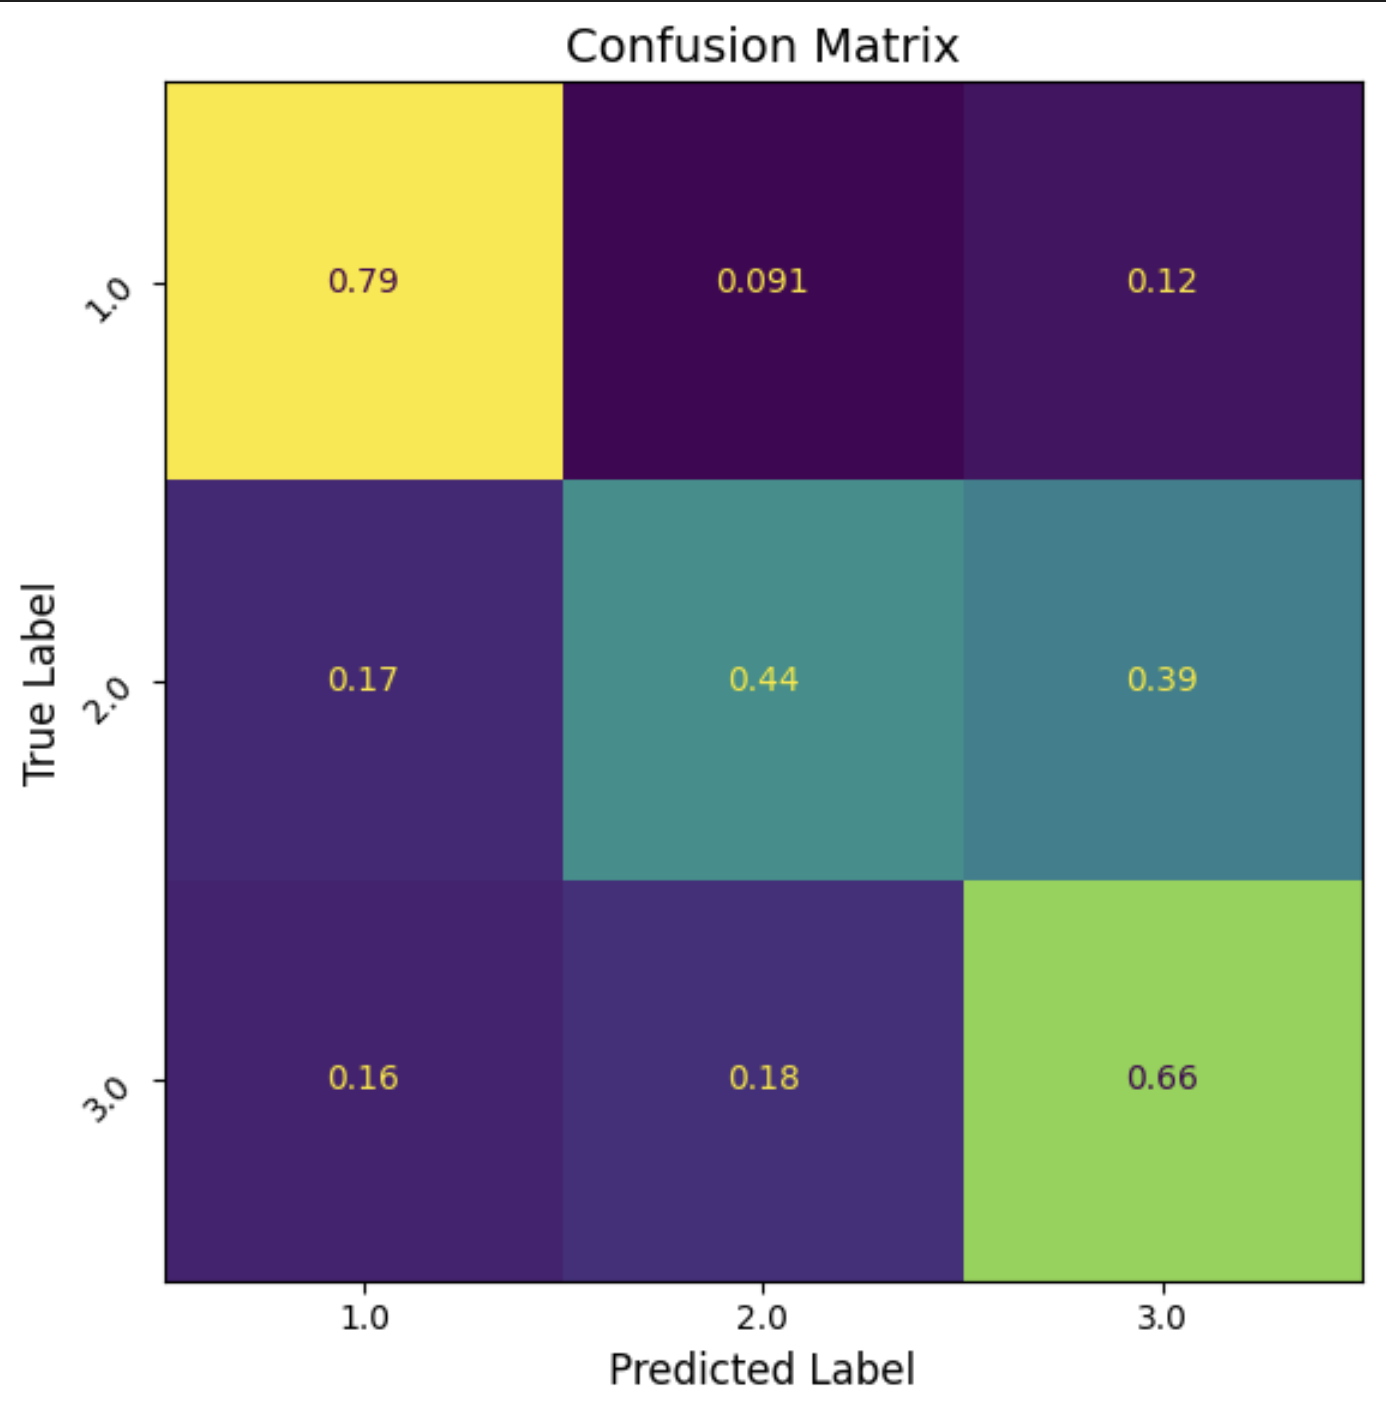
\includegraphics[width=\columnwidth,height=0.75\columnwidth,keepaspectratio]{screen_results/confusion_matrix_stacking_s.png}
\end{minipage}
\end{center}

\subsection*{Voting (Smoke)}
\begin{center}
\begin{minipage}[c]{0.50\columnwidth}
\resizebox{\columnwidth}{!}{%
\begin{tabular}{lcccc}
\toprule
Label        & Precision & Recall & F1-score & Support \\
\midrule
Non-smoker   & 0.93      & 0.74   & 0.83     & 111686 \\
Ex-smoker    & 0.43      & 0.53   & 0.47     & 31585  \\
Smoker       & 0.48      & 0.66   & 0.56     & 39049  \\
\midrule
Accuracy     & --        & --     & 0.69     & 182320 \\
Macro avg    & 0.61      & 0.65   & 0.62     & 182320 \\
Weighted avg & 0.75      & 0.69   & 0.71     & 182320 \\
\bottomrule
\end{tabular}%
}
\end{minipage}\hspace{\columnsep}%
\begin{minipage}[c]{0.40\columnwidth}
\centering
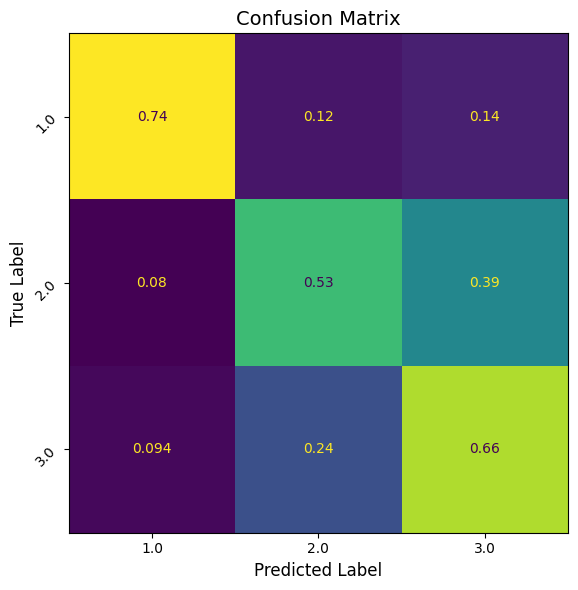
\includegraphics[width=\columnwidth,height=0.75\columnwidth,keepaspectratio]{screen_results/confusion_matrix_voting_s.png}
\end{minipage}
\end{center}

\subsection*{Stacking (Drink)}
\begin{center}
\begin{minipage}[c]{0.50\columnwidth}
\resizebox{\columnwidth}{!}{%
\begin{tabular}{lcccc}
\toprule
Label & Precision & Recall & F1-score & Support \\
\midrule
Y     & 0.73      & 0.71   & 0.72     & 90360 \\
N     & 0.72      & 0.74   & 0.73     & 91960 \\
\midrule
Accuracy     & --        & --     & 0.73     & 182320 \\
Macro avg    & 0.73      & 0.73   & 0.73     & 182320 \\
Weighted avg & 0.73      & 0.73   & 0.73     & 182320 \\
\bottomrule
\end{tabular}%
}
\end{minipage}\hspace{\columnsep}%
\begin{minipage}[c]{0.40\columnwidth}
\centering
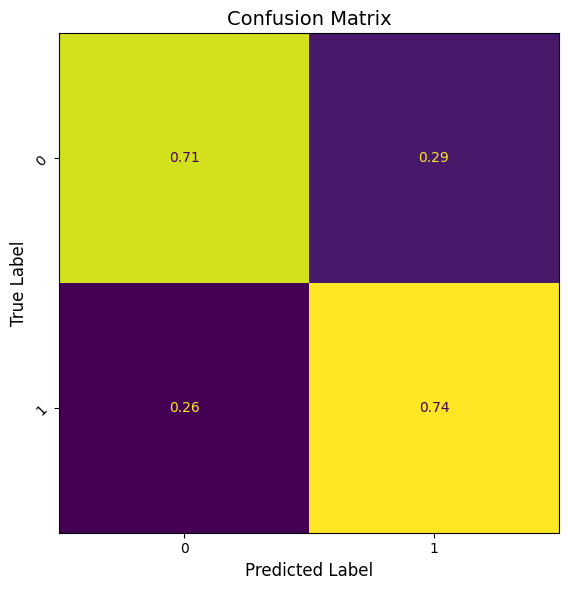
\includegraphics[width=\columnwidth,height=0.75\columnwidth,keepaspectratio]{screen_results/confusion_matrix_stacking_d.png}
\end{minipage}
\end{center}

\subsection*{Voting (Drink)}
\begin{center}
\begin{minipage}[c]{0.50\columnwidth}
\resizebox{\columnwidth}{!}{%
\begin{tabular}{lcccc}
\toprule
Label & Precision & Recall & F1-score & Support \\
\midrule
Y     & 0.74      & 0.68   & 0.71     & 90360 \\
N     & 0.71      & 0.76   & 0.73     & 91960 \\
\midrule
Accuracy     & --        & --     & 0.72     & 182320 \\
Macro avg    & 0.72      & 0.72   & 0.72     & 182320 \\
Weighted avg & 0.72      & 0.72   & 0.72     & 182320 \\
\bottomrule
\end{tabular}%
}
\end{minipage}\hspace{\columnsep}%
\begin{minipage}[c]{0.40\columnwidth}
\centering
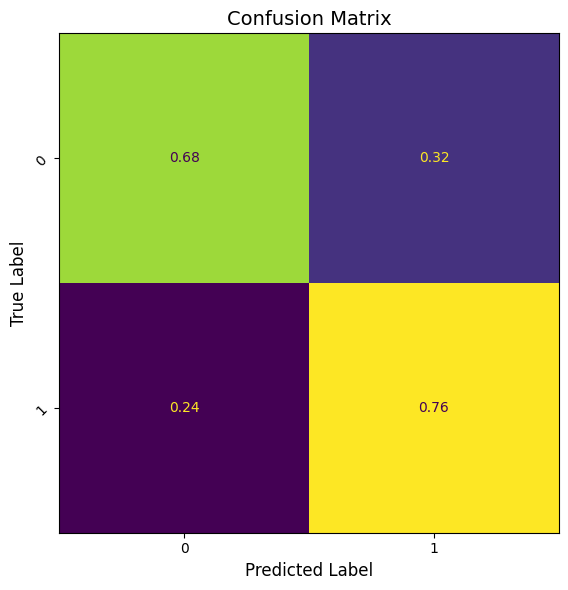
\includegraphics[width=\columnwidth,height=0.75\columnwidth,keepaspectratio]{screen_results/confusion_matrix_voting_d.png}
\end{minipage}
\end{center}

%%%%%%%%%%%%%%%%%%%%%%%%%%%%%%%%%%%%%%%%%%%%%%%%%%%%%%%%%%%%%%%%%%%%%%%%%%%%%%
% Classificatore Gerarchico (Smoke)
%%%%%%%%%%%%%%%%%%%%%%%%%%%%%%%%%%%%%%%%%%%%%%%%%%%%%%%%%%%%%%%%%%%%%%%%%%%%%%

\subsection{Classificatore Gerarchico (Smoke)}
Per quanto riguarda la classificazione sul fumo, che alla fine è stato al centro del nostro progetto più della classificazione sull'alcool, abbiamo fatto un ultimo tentativo per cercare di ottenere un modello di predizione che migliorasse le metriche ottenute fino a questo punto, implementando un classificatore gerarchico; purtoppo, come già accennato nella sezione relativa alla spiegazione dei modelli utilizzati nel progetto non siamo riusciti nel nostro intento per verie ragioni, anche se il risultato finale si avvicina molto alle performance ottenute dal modello Random Forest.
C'è però da fare una precisazione: nonostante questo modello di classificazione gerarchica non sia stato creato come era nostro intento, siamo convinti che la filosofia di creare un modello predittivo di questo tipo sia la carta vincente per poter ottenere il miglior modello possibile per questo tipo di dataset.
Idealmente, infatti, allenando prima un modello che separi nel miglior modo possibile le classi "Non-fumatore" e "Ex-fumatore o Fumatore" ed in un secondo momento un modello che sappia separare meglio possibile le classi "Ex-fumatore" e "Fumatore" si dovrebbe riuscire ad ottenere una "pipeline" che sia in grado di occuparsi step by step della suddivisione dei sample.



\subsection*{Stage 1 --- Non-smokers vs. Ex-/Smokers}
\begin{center}
\begin{minipage}[c]{0.50\columnwidth}
\resizebox{\columnwidth}{!}{%
\begin{tabular}{lcccc}
\toprule
Label         & Precision & Recall & F1-score & Support \\
\midrule
Non-smoker    & 0.93      & 0.75   & 0.83     & 111686 \\
Ex-/Smokers   & 0.69      & 0.91   & 0.79     & 70634  \\
\midrule
Accuracy     & --        & --     & 0.81     & 182320 \\
Macro avg    & 0.81      & 0.83   & 0.81     & 182320 \\
Weighted avg & 0.84      & 0.81   & 0.81     & 182320 \\
\bottomrule
\end{tabular}%
}
\end{minipage}\hspace{\columnsep}%
\begin{minipage}[c]{0.40\columnwidth}
\centering
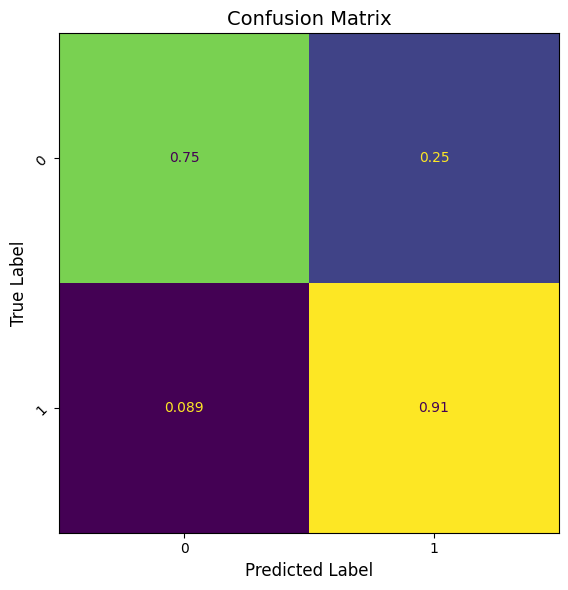
\includegraphics[width=\columnwidth,height=0.75\columnwidth,keepaspectratio]{screen_results/confusion_matrix_separation1.png}
\end{minipage}
\end{center}

\subsection*{Stage 2 --- Ex-smokers vs. Smokers}
\begin{center}
\begin{minipage}[c]{0.50\columnwidth}
\resizebox{\columnwidth}{!}{%
\begin{tabular}{lcccc}
\toprule
Label      & Precision & Recall & F1-score & Support \\
\midrule
Ex-smoker  & 0.62      & 0.60   & 0.61     & 31585  \\
Smoker     & 0.68      & 0.71   & 0.70     & 39049  \\
\midrule
Accuracy     & --        & --     & 0.66     & 70634  \\
Macro avg    & 0.65      & 0.65   & 0.65     & 70634  \\
Weighted avg & 0.66      & 0.66   & 0.66     & 70634  \\
\bottomrule
\end{tabular}%
}
\end{minipage}\hspace{\columnsep}%
\begin{minipage}[c]{0.40\columnwidth}
\centering
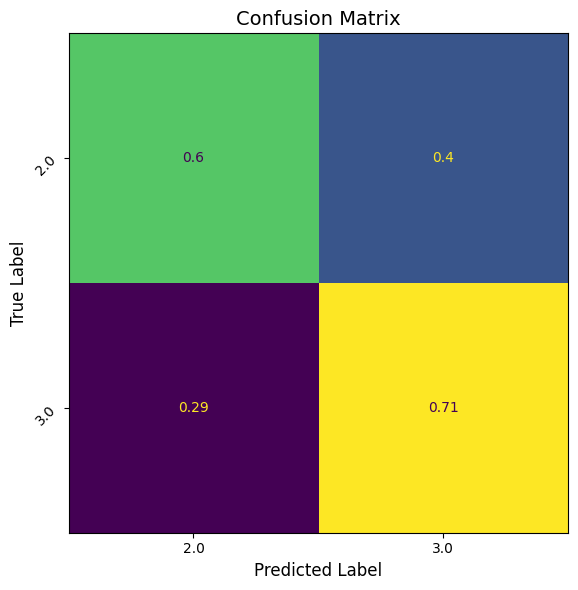
\includegraphics[width=\columnwidth,height=0.75\columnwidth,keepaspectratio]{screen_results/confusion_matrix_separation2.png}
\end{minipage}
\end{center}

\subsection*{Test Classificatore Gerarchico}
\begin{center}
\begin{minipage}[c]{0.50\columnwidth}
\resizebox{\columnwidth}{!}{%
\begin{tabular}{lcccc}
\toprule
Label        & Precision & Recall & F1-score & Support \\
\midrule
Non-smoker   & 0.94      & 0.73   & 0.82     & 111704 \\
Ex-smoker    & 0.41      & 0.55   & 0.47     & 31616  \\
Smoker       & 0.48      & 0.65   & 0.55     & 39085  \\
\midrule
Accuracy     & --        & --     & 0.68     & 182405 \\
Macro avg    & 0.61      & 0.64   & 0.61     & 182405 \\
Weighted avg & 0.75      & 0.68   & 0.70     & 182405 \\
\bottomrule
\end{tabular}%
}
\end{minipage}\hspace{\columnsep}%
\begin{minipage}[c]{0.40\columnwidth}
\centering
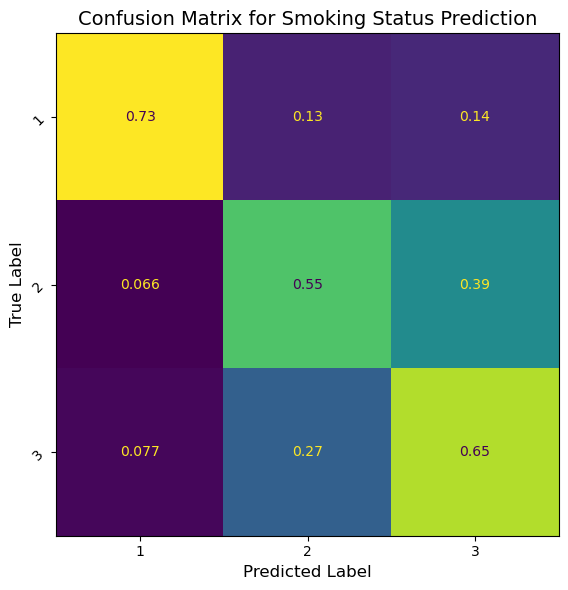
\includegraphics[width=\columnwidth,height=0.75\columnwidth,keepaspectratio]{screen_results/confusion_matrix_multistep_s.png}
\end{minipage}
\end{center}

\newpage

\subsection{Visualizzazione della Separazione delle Classi}

Di seguito vengono riportate le distribuzioni nello spazio dei dati presenti nel dataset, ottenuti sfruttando le tecniche di t-SNE e PCA; in questo modo abbiamo potuto visualizzare quanto effettivamente le classi del nostro dataset fossero sovrapposte tra di loro. 
Ovviamente per rendere il tutto più comprensibile, abbiamo "plottato" il tutto in uno spazio a 2 dimensioni e considerando in un primo momento le label "Non-fumatore" e "Ex-fumatore o Fumatore" accorpate in una unica classe ed in un secondo momento le classi "Ex-fumatore" e "Fumatore". 
Come si può vedere, la divisione "Non-fumatore" e "Ex-fumatore o Fumatore" è abbastanza marcata e facile da individuare, mentre per l'altra divisione si nota una netta sovrapposizione dei dati delle due classi, marcando dunque la difficoltà nel riuscire a distinguere in maniera anche solo parziale le due classi. 
Per ottenere risultati in tempi contenuti, abbiamo utilizzato solo il 10\% del dataset.

\begin{figure}[h]
    \centering
    \begin{minipage}{0.45\textwidth}
        \centering
        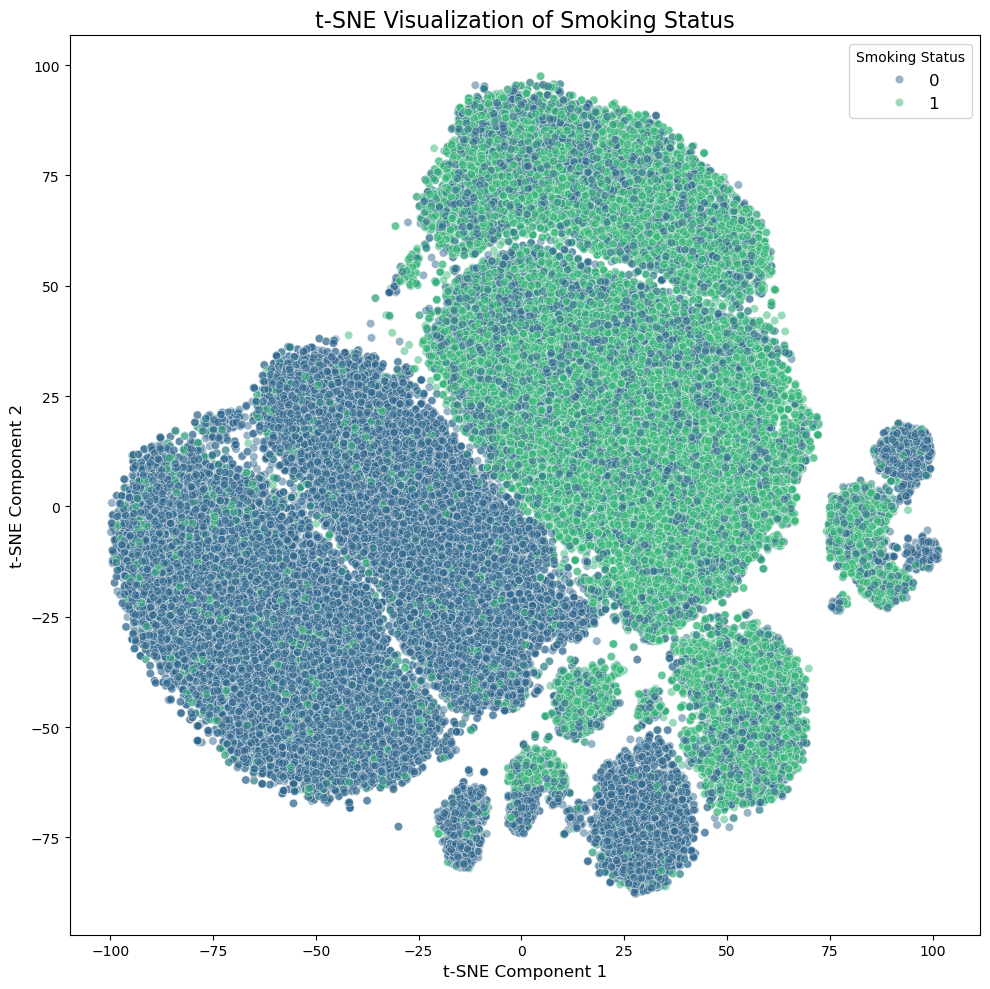
\includegraphics[width=\textwidth]{screen_results/tSNE_smoking_non_smoking.png}
        \caption{t-SNE "Non-fumatore" e "Ex-fumatore o Fumatore"}
    \end{minipage}
    \hfill
    \begin{minipage}{0.45\textwidth}
        \centering
        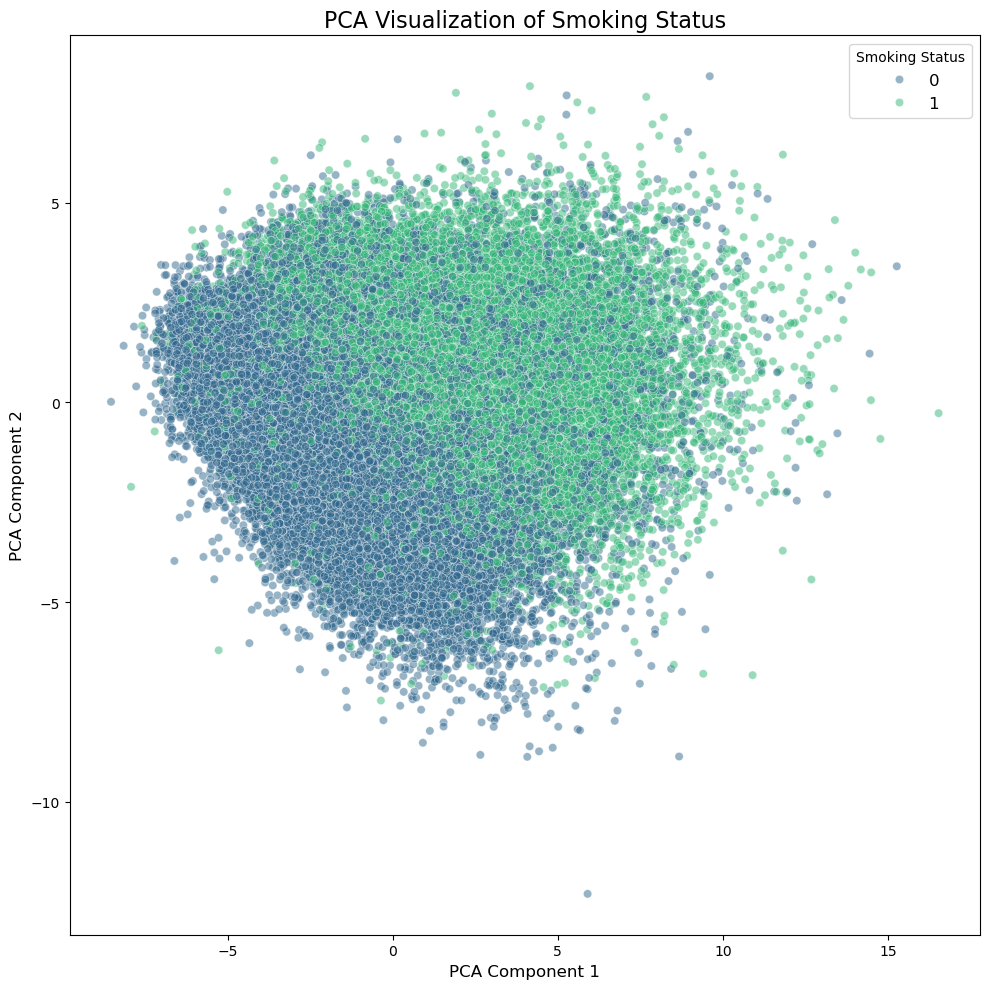
\includegraphics[width=\textwidth]{screen_results/pca_smoking_non_smoking.png}
        \caption{PCA "Non-fumatore" e "Ex-fumatore o Fumatore"}
    \end{minipage}
\end{figure}

\begin{figure}[h]
    \centering
    \begin{minipage}{0.45\textwidth}
        \centering
        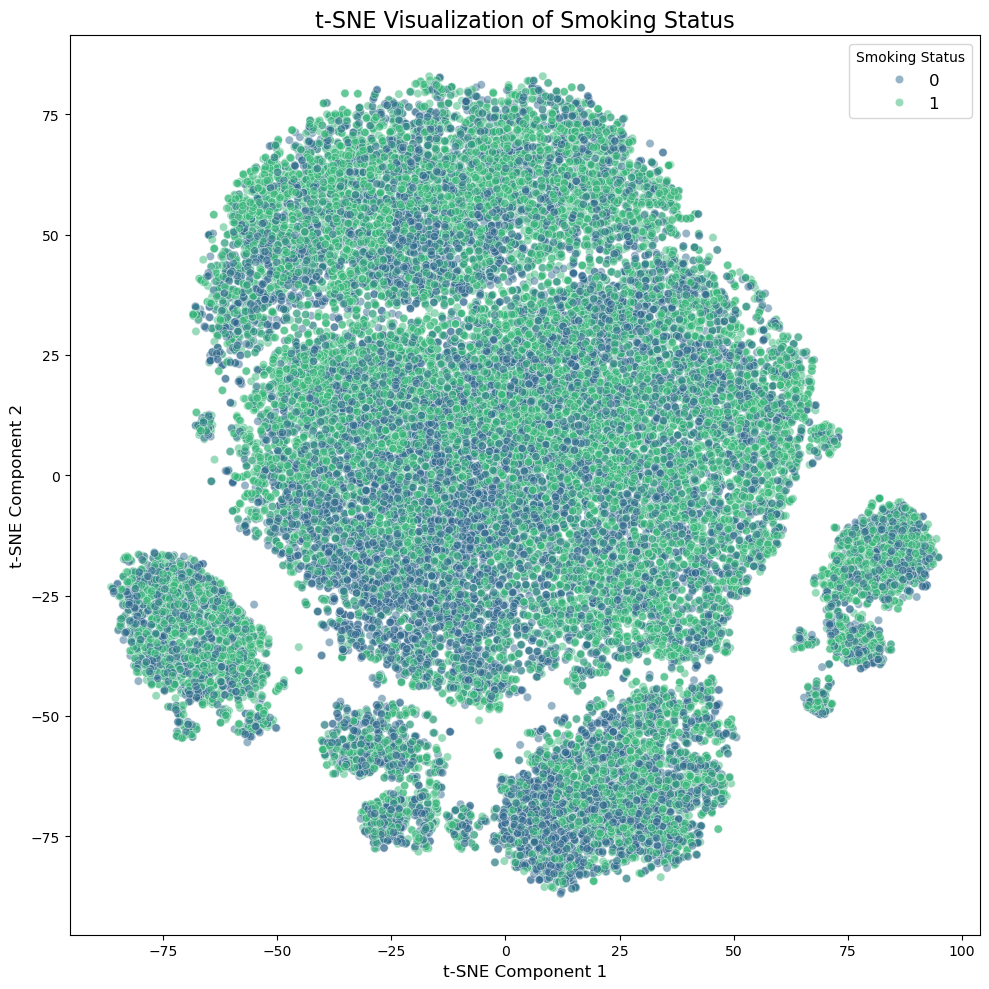
\includegraphics[width=\textwidth]{screen_results/tSNE_smoking_ex_smoking.png}
        \caption{t-SNE "Ex-fumatore" e "Fumatore"}
    \end{minipage}
    \hfill
    \begin{minipage}{0.45\textwidth}
        \centering
        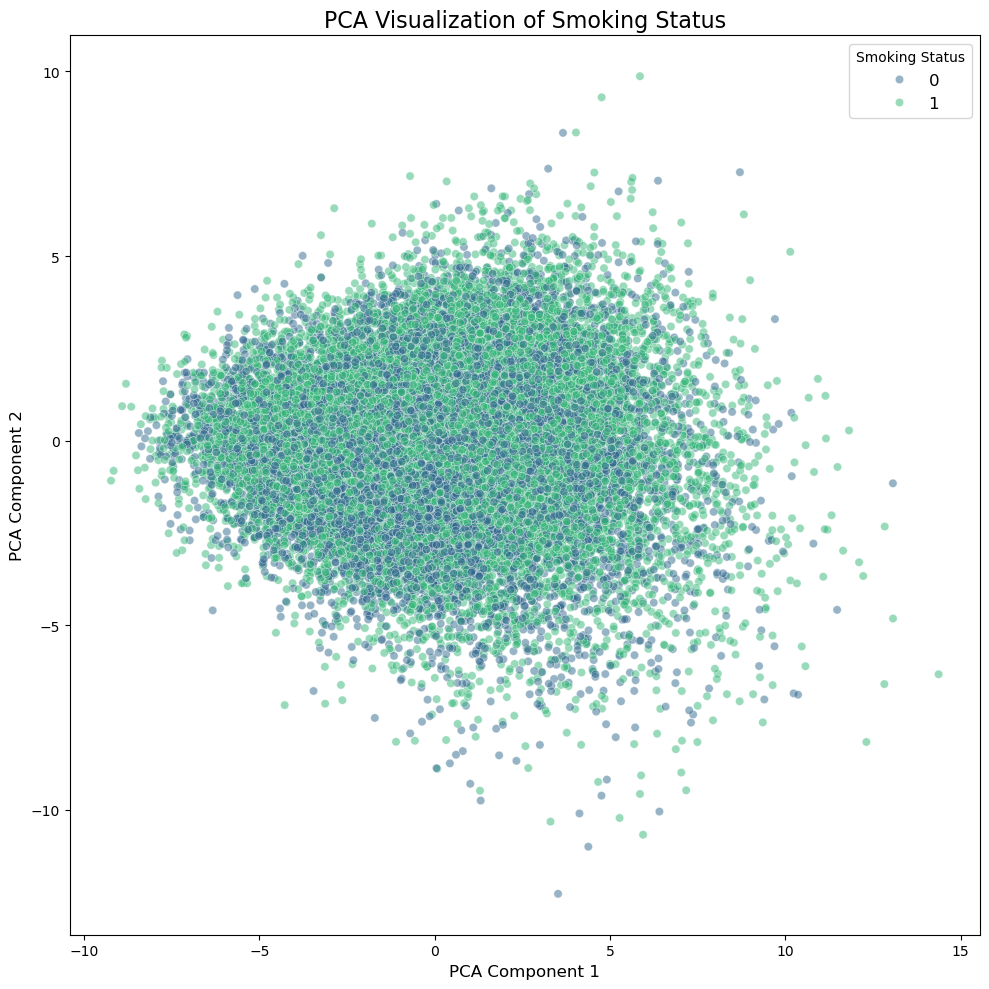
\includegraphics[width=\textwidth]{screen_results/pca_smoking_ex_smoking.png}
        \caption{PCA "Ex-fumatore" e "Fumatore"}
    \end{minipage}
\end{figure}